% Options for packages loaded elsewhere
\PassOptionsToPackage{unicode}{hyperref}
\PassOptionsToPackage{hyphens}{url}
\PassOptionsToPackage{dvipsnames,svgnames*,x11names*}{xcolor}
%
\documentclass[
  12pt,
]{article}
\usepackage{lmodern}
\usepackage{amsmath}
\usepackage{ifxetex,ifluatex}
\ifnum 0\ifxetex 1\fi\ifluatex 1\fi=0 % if pdftex
  \usepackage[T1]{fontenc}
  \usepackage[utf8]{inputenc}
  \usepackage{textcomp} % provide euro and other symbols
  \usepackage{amssymb}
\else % if luatex or xetex
  \usepackage{unicode-math}
  \defaultfontfeatures{Scale=MatchLowercase}
  \defaultfontfeatures[\rmfamily]{Ligatures=TeX,Scale=1}
  \setmainfont[]{Times New Roman}
\fi
% Use upquote if available, for straight quotes in verbatim environments
\IfFileExists{upquote.sty}{\usepackage{upquote}}{}
\IfFileExists{microtype.sty}{% use microtype if available
  \usepackage[]{microtype}
  \UseMicrotypeSet[protrusion]{basicmath} % disable protrusion for tt fonts
}{}
\makeatletter
\@ifundefined{KOMAClassName}{% if non-KOMA class
  \IfFileExists{parskip.sty}{%
    \usepackage{parskip}
  }{% else
    \setlength{\parindent}{0pt}
    \setlength{\parskip}{6pt plus 2pt minus 1pt}}
}{% if KOMA class
  \KOMAoptions{parskip=half}}
\makeatother
\usepackage{xcolor}
\IfFileExists{xurl.sty}{\usepackage{xurl}}{} % add URL line breaks if available
\IfFileExists{bookmark.sty}{\usepackage{bookmark}}{\usepackage{hyperref}}
\hypersetup{
  colorlinks=true,
  linkcolor=RoyalBlue,
  filecolor=Maroon,
  citecolor=Blue,
  urlcolor=RoyalBlue,
  pdfcreator={LaTeX via pandoc}}
\urlstyle{same} % disable monospaced font for URLs
\usepackage[margin=1in]{geometry}
\usepackage{graphicx}
\makeatletter
\def\maxwidth{\ifdim\Gin@nat@width>\linewidth\linewidth\else\Gin@nat@width\fi}
\def\maxheight{\ifdim\Gin@nat@height>\textheight\textheight\else\Gin@nat@height\fi}
\makeatother
% Scale images if necessary, so that they will not overflow the page
% margins by default, and it is still possible to overwrite the defaults
% using explicit options in \includegraphics[width, height, ...]{}
\setkeys{Gin}{width=\maxwidth,height=\maxheight,keepaspectratio}
% Set default figure placement to htbp
\makeatletter
\def\fps@figure{htbp}
\makeatother
\setlength{\emergencystretch}{3em} % prevent overfull lines
\providecommand{\tightlist}{%
  \setlength{\itemsep}{0pt}\setlength{\parskip}{0pt}}
\setcounter{secnumdepth}{-\maxdimen} % remove section numbering
\usepackage{setspace}\doublespacing
\usepackage[left]{lineno}
\ifluatex
  \usepackage{selnolig}  % disable illegal ligatures
\fi
\newlength{\cslhangindent}
\setlength{\cslhangindent}{1.5em}
\newlength{\csllabelwidth}
\setlength{\csllabelwidth}{3em}
\newenvironment{CSLReferences}[2] % #1 hanging-ident, #2 entry spacing
 {% don't indent paragraphs
  \setlength{\parindent}{0pt}
  % turn on hanging indent if param 1 is 1
  \ifodd #1 \everypar{\setlength{\hangindent}{\cslhangindent}}\ignorespaces\fi
  % set entry spacing
  \ifnum #2 > 0
  \setlength{\parskip}{#2\baselineskip}
  \fi
 }%
 {}
\usepackage{calc}
\newcommand{\CSLBlock}[1]{#1\hfill\break}
\newcommand{\CSLLeftMargin}[1]{\parbox[t]{\csllabelwidth}{#1}}
\newcommand{\CSLRightInline}[1]{\parbox[t]{\linewidth - \csllabelwidth}{#1}\break}
\newcommand{\CSLIndent}[1]{\hspace{\cslhangindent}#1}

\author{}
\date{\vspace{-2.5em}}

\begin{document}

\pagenumbering{arabic}

Running head: Burn severity and the grass fire cycle

Title: Burn severity, fuel connectivity and seed bank survivorship drive
the annual-grass fire cycle in a semi-arid shrubland.

Adam L. Mahood\textsuperscript{1,2,\texttt{*}}, Michael J.
Koontz\textsuperscript{2}, Jennifer K. Balch\textsuperscript{1,2}

\small

\textsuperscript{1} Department of Geography, University of Colorado
Boulder, Boulder, CO, USA

\textsuperscript{2} Earth Lab, University of Colorado, Boulder, CO, USA

\texttt{*} Corresponding author:
\href{mailto:admahood@gmail.com}{\nolinkurl{admahood@gmail.com}}

\normalsize

\linenumbers

\hypertarget{abstract}{%
\subsection{Abstract}\label{abstract}}

Introduced grasses can initiate novel grass-fire cycles that alter
ecosystem structure and function, and threaten biodiversity. In
sagebrush communities in the western United States, annual grass
invasion increases the connectivity of fine fuels, which increases the
size and spatial contiguity of fires. This increase in fire size and
contiguity results in post-fire plant communities that are dominated by
introduced annual grasses (IAG), which are themselves more likely to
promote large fires and initiate a novel grass-fire cycle. But the
mechanisms by which pre-fire invasion and fire occurrence are linked to
higher post-fire flammability are not fully understood.

Here, we used total vegetation cover (TVC) as a proxy for fuel
connectivity and found that pre-fire TVC increased burn severity. We
then used a Bayesian joint species distribution model to examine how
burn severity affected the proportion of IAG in the seed bank, and found
that higher burn severity had mostly positive or neutral effects on the
occurrence of IAG and other non-native species, and mostly negative or
neutral relationships with native species. To complete the positive
feedback loop, we found that the abundance of IAG seeds in the seedbank
immediately post-fire had a positive effect on the fuel connectivity 3
years after fire. This is the first study that we are aware of in the
western US that shows how burn severity influences seed bank species
composition, as well as examining the full feedback loop between fuel
connectivity, burn severity and seed bank species composition. These
results suggest that measurable characteristics of ecosystem structure
(e.g.~TVC) and fire (dNBR) may be used to inform management actions to
mitigate the negative effects of the grass-fire cycle, perhaps via
targeted restoration applications or pre-fire fuel treatments.

\emph{Keywords}: cheatgrass, sagebrush, grass-fire cycle, joint species
distribution model, burn severity, fuel connectivity, \emph{Bromus
tectorum}, \emph{Artemisia tridentata}

\hypertarget{introduction}{%
\subsection{1. Introduction}\label{introduction}}

One of the consequences of global change in the 21\(^\text{st}\) century
that is most difficult to reverse is when ecosystems abruptly shift from
one stable species assemblage to another
(\protect\hyperlink{ref-Ratajczak2018}{Ratajczak et al. 2018}). In
tropical ecosystems, three alternative stable states have been
identified along a gradient of precipitation: forests, savannas and
grasslands (\protect\hyperlink{ref-Hirota2011}{Hirota et al. 2011};
\protect\hyperlink{ref-Staver2011}{Staver, Archibald, and Levin 2011}).
These three states cluster around values of tree cover (approximately
80, 30 and 0 percent) that occur among overlapping levels of
precipitation, and so it is thought that internal, self-reinforcing
mechanisms maintain these alternate states
(\protect\hyperlink{ref-Andersen2009}{Andersen et al. 2009}). In the
forested state there is a self-reinforcing positive feedback between
evapotranspiration and tree cover
(\protect\hyperlink{ref-Staal2020}{Staal et al. 2020}). In the grassland
and savanna states, there are feedbacks between grass flammability and
fire occurrence (The grass-fire cycle,
\protect\hyperlink{ref-DAntonio1992}{D'Antonio and Vitousek 1992};
\protect\hyperlink{ref-Staver2011}{Staver, Archibald, and Levin 2011}).

A classic example of a novel grass-fire cycle in a semi-arid, temperate
system is the invasion and persistence of \emph{Bromus tectorum} L. and
other introduced annual grasses in the Great Basin of the western United
States. Here, over half of Wyoming big sagebrush (\emph{Artemisia
tridentata} ssp. \emph{wyomingensis} Beetle \& Young) ecosystems have
been degraded, fragmented or lost completely
(\protect\hyperlink{ref-Davies2011}{Davies et al. 2011}). This has been
attributed to a host of causes, including wildfire
(\protect\hyperlink{ref-Balch2013}{Balch et al. 2013}), grazing
(\protect\hyperlink{ref-Williamson2019}{Williamson et al. 2019}), land
use/land cover change, and the invasion of annual grasses. At uninvaded
sites, the space between shrubs is typically composed of bare ground
covered in biological soil crust and dotted with perennial bunch
grasses. The lack of fuel connectivity is believed to limit fire spread,
with a historical fire regime of infrequent, patchy fires
(\protect\hyperlink{ref-Baker2006}{Baker 2006};
\protect\hyperlink{ref-Bukowski2013}{Bukowski and Baker 2013};
\protect\hyperlink{ref-Keeley2019}{Keeley and Pausas 2019}). Annual
grass invasion increases fuel connectivity while decreasing fuel
moisture (\protect\hyperlink{ref-Davies2013}{Davies and Nafus 2013}),
leading to increased fire size and frequency
(\protect\hyperlink{ref-Whisenant1990}{Whisenant 1990};
\protect\hyperlink{ref-Knapp1996}{Knapp 1996};
\protect\hyperlink{ref-Balch2013}{Balch et al. 2013}). After fire, the
landscape is often dominated by introduced annual grasses and forbs. But
in order to understand how the grassland state persists, the mechanisms
by which fire benefits the introduced annual grass must be understood.
\protect\hyperlink{ref-Petraitis1999}{Petraitis and Latham}
(\protect\hyperlink{ref-Petraitis1999}{1999}) posited that the
maintenance of alternate species assemblages requires first a
disturbance that removes the species from the initial assemblage and
second the arrival of the species of the alternate assemblage. One
understudied mechanism that may explain both is the interaction between
burn severity and the species composition of the soil seed bank.

The relationship between the species composition of the seed bank and
fire severity and/or intensity is relatively understudied. In different
systems, individual species have adapted strategies to cope with fires
that may be adapted to different severities. In boreal forests, the
depth of the burn may be more important more than the temperature of the
fire, with species-specific effects on recovery depending on whether the
species recovers via resprouting or from the seed bank
(\protect\hyperlink{ref-Morgan1988}{Morgan and Neuenschwander 1988};
\protect\hyperlink{ref-Schimmel1996}{Schimmel and Granström 1996}). In a
wetland study in Japan, high severity fire was found to increase
seedbank diversity, and the similarity between the seedbank composition
and aboveground composition was higher in places burned at high severity
(\protect\hyperlink{ref-Kimura2011}{Kimura and Tsuyuzaki 2011}). There
have been a handful of studies in temperate, semi-arid regions.
\protect\hyperlink{ref-Lipoma2018}{Lipoma, Funes, and Díaz}
(\protect\hyperlink{ref-Lipoma2018}{2018}) found that in shrubland
high-severity fire reduced the overall number of seeds in the seedbank
but did not change the floristic or functional composition.
\protect\hyperlink{ref-Maia2012}{Maia et al.}
(\protect\hyperlink{ref-Maia2012}{2012}) found intraspecific differences
in post-fire seedbank densities that were explained by burn severity in
a pine plantation in Portugal.
\protect\hyperlink{ref-Palmer2018}{Palmer, Denham, and Ooi}
(\protect\hyperlink{ref-Palmer2018}{2018}) found that the residual
seedbank after fire varied with severity between two \emph{Acacia}
species in Australia. \protect\hyperlink{ref-Wright2016}{Wright, Latz,
and Zuur} (\protect\hyperlink{ref-Wright2016}{2016}) found that
Australian mulga (\emph{Acacia aneura}) had higher regeneration after
higher fire temperatures. In Iran,
\protect\hyperlink{ref-Heydari2017}{Heydari et al.}
(\protect\hyperlink{ref-Heydari2017}{2017}) found that low-severity fire
increased diversity in the soil seed bank, but high-severity fire led to
losses. These studies show that the effects of fire severity on the seed
bank are ecosystem- and species-specific. High severity fire can benefit
species that use the seedbank (\protect\hyperlink{ref-Kimura2011}{Kimura
and Tsuyuzaki 2011}), be seedbank-neutral
(\protect\hyperlink{ref-Lipoma2018}{Lipoma, Funes, and Díaz 2018}), or
have a negative effect (\protect\hyperlink{ref-Heydari2017}{Heydari et
al. 2017}). Furthermore, beyond simply affecting seed mortality, fire
temperature can also alter physical seed dormancy thresholds
(\protect\hyperlink{ref-Liyanage2017}{Liyanage and Ooi 2017}).

In order for an annual like \emph{B. tectorum} it to benefit from fire,
which it clearly does (\protect\hyperlink{ref-Balch2013}{Balch et al.
2013}; \protect\hyperlink{ref-Mahood2019}{Mahood and Balch 2019}), it
would need enough seeds in the post-fire landscape to achieve a fitness
benefit and become well-represented in the post-fire plant assemblage
(\protect\hyperlink{ref-Bond1995}{Bond and Midgley 1995}). If the fire
is patchy, this can happen through post-fire seed dispersal, and
\emph{B. tectorum} seeds have been shown to have increased dispersal
distances after fire (\protect\hyperlink{ref-Monty2013}{Monty, Brown,
and Johnston 2013}). Without unburned patches, seeds must survive the
fire. There is strong evidence that \emph{B. tectorum} builds a
well-stocked pool of seeds in the soil and litter, even when it is not
well represented in the above-ground plant assemblage
(\protect\hyperlink{ref-Young1975}{Young and Evans 1975};
\protect\hyperlink{ref-Hassan1986}{Hassan and West 1986};
\protect\hyperlink{ref-Boudell2002}{Boudell, Link, and Johansen 2002}).
If the increase in fuel connectivity caused by \emph{B. tectorum}
increases the severity of fire, it stands to reason that burn severity
would influence the community composition of the post-fire seed bank in
a way that facilitates the post-fire dominance of \emph{B. tectorum}. To
our knowledge, despite several studies on the relationship between fire
and the seed bank in this system
(\protect\hyperlink{ref-Young1975}{Young and Evans 1975};
\protect\hyperlink{ref-Hassan1986}{Hassan and West 1986};
\protect\hyperlink{ref-Humphrey2001}{Humphrey and Schupp 2001};
\protect\hyperlink{ref-Boudell2002}{Boudell, Link, and Johansen 2002};
\protect\hyperlink{ref-Barga2018}{Barga and Leger 2018}), no studies to
date have examined this potential effect of burn severity on the seed
bank.

There is strong evidence that \emph{B. tectorum} invasion alters the
physical properties of fire, including fire temperature
(\protect\hyperlink{ref-Brooks2004}{Brooks et al. 2004};
\protect\hyperlink{ref-Jones2015}{Jones et al. 2015}) and burn severity
(defined here as the proportion of biomass burned
(\protect\hyperlink{ref-Keeley2009}{Keeley 2009})). Burn severity can be
measured after fire \emph{in situ}, or estimated from satellite images
by comparing scenes from before and after the fire
(\protect\hyperlink{ref-Miller2009}{J. D. Miller et al. 2009}). While in
many cases fires that burn at higher temperatures will also burn at
higher severities, grass fires may not always have such a relationship.
Direct measurements have shown that \emph{B. tectorum} burns at low
temperatures (\protect\hyperlink{ref-Beckstead2011}{Beckstead et al.
2011}; \protect\hyperlink{ref-Germino2016}{Germino, Chambers, and Brown
2016}). Because fire duration is inversely related to soil heating,
lower fire temperatures can be inferred from the commonly observed
phenomenon that \emph{B. tectorum}-fueled fires burn fast. Soil heating
affects the response of vegetation to fire
(\protect\hyperlink{ref-Gagnon2015}{Gagnon et al. 2015}), including the
capacity of the seeds of \emph{B. tectorum} to remain viable after fire
(\protect\hyperlink{ref-Humphrey2001}{Humphrey and Schupp 2001}).
Because \emph{B. tectorum} also increases horizontal fuel connectivity
(\protect\hyperlink{ref-Davies2013}{Davies and Nafus 2013}), this leads
to more contiguously burned areas with fewer unburned plants, and
therefore higher burn severity, despite lower fire temperatures.

If increased burn severity is a mechanism by which \emph{B. tectorum}
invasion excludes native plants in sagebrush shrublands, then an area
with high burn severity should have a lower occurrence of viable seeds
of native species, and a higher occurrence of the seeds of fire-tolerant
introduced annual plants. This would lead to the dominance of introduced
annual grasses and forbs and would result in higher fuel connectivity,
closing the positive feedback loop. Prior work has demonstrated that
\emph{A. tridentata} communities have historically had long fire
rotations (\textgreater150 years)
(\protect\hyperlink{ref-Baker2006}{Baker 2006};
\protect\hyperlink{ref-Bukowski2013}{Bukowski and Baker 2013}). Plants
that are adapted to infrequent fire would be unlikely to produce seeds
that are adapted to surviving fire, or dispersal mechanisms to take
advantage of the resources available immediately after fire
(\protect\hyperlink{ref-Davis2000}{Davis et al. 2000};
\protect\hyperlink{ref-Keeley2011}{Keeley et al. 2011}). \emph{A.
tridentata} relies on tolerating drought and opportunistically devoting
its resources to producing large seed crops in cool, wet years
(\protect\hyperlink{ref-Meyer1994}{Meyer 1994};
\protect\hyperlink{ref-Perryman2001}{Perryman et al. 2001};
\protect\hyperlink{ref-Shriver2018}{Shriver et al. 2018}). When it burns
it burns with high intensity, killing individual plants, and the
remaining unburned neighbors seed the area (\emph{sensu}
\protect\hyperlink{ref-Schwilk2002}{Schwilk and Kerr 2002}). The seeds
have a short dispersal distance, the vast majority falling within a few
meters of the parent plant (\protect\hyperlink{ref-Meyer1994}{Meyer
1994}; \protect\hyperlink{ref-Schlaepfer2014}{Schlaepfer, Lauenroth, and
Bradford 2014}). They typically lose their viability after one growing
season if they remain on the soil surface or under litter, but can
remain viable for at least two years if they are buried under a few
inches of soil (\protect\hyperlink{ref-Wijayratne2009}{Wijayratne and
Pyke 2009}).

The Great Basin has not escaped the recent warming and drying trend that
the western U.S. has experienced
(\protect\hyperlink{ref-Melillo2014}{Melillo, Richmond, and Yohe 2014};
\protect\hyperlink{ref-Bradford2020}{Bradford et al. 2020}). This is
expected to affect \emph{A. tridentata} directly by decreasing
germination and seedling survival, and indirectly by causing the plants
to produce lighter seeds
(\protect\hyperlink{ref-Schlaepfer2014}{Schlaepfer, Lauenroth, and
Bradford 2014}). With this in mind, there is another potential
self-reinforcing mechanism that could serve to maintain the high fuel
connectivity state without fire. That is that the post-fire state with
high fuel connectivity is associated with two mechanisms for competitive
exclusion of natives. First, it reduces soil moisture which is
unfavorable for \emph{Artemisia} seedlings
(\protect\hyperlink{ref-Turnbull2012}{Turnbull et al. 2012};
\protect\hyperlink{ref-Wilcox2012}{Wilcox et al. 2012}). Second, the
dominant plant, \emph{B. tectorum}, can out-compete native plants for
early spring moisture (\protect\hyperlink{ref-Meyer1994}{Meyer 1994};
\protect\hyperlink{ref-Chambers2007}{Chambers et al. 2007}).

Here, we collected soil cores from 14 locations along the perimeter of a
large fire (the Hot Pot fire, \textasciitilde50,000 ha) immediately
after it was extinguished, in northern Nevada in July 2016. Because it
burned a large area in only three days, we could sample a broad area
while being reasonably certain that the climatic conditions during the
fire were the same at all sites. Because we collected our samples
immediately after the fire was extinguished, we felt confident that the
seed bank samples did not contain seeds deposited by post-fire
dispersal. We put the samples in cold storage and germinated the seeds
from those cores in a greenhouse the following spring. In spring 2017
and fall 2019 we collected information on vegetation structure and
diversity at each location. We hypothesized that (H1) Pre-fire fuel
connectivity would be positively related to burn severity; (H2) burn
severity would increase the occurrence probability of introduced annual
species in the seed bank and reduce the occurrence probability of native
species; (H2a) increased fuel connectivity brought on by the invasion of
annual grasses already depleted the diversity of the soil seed bank
before the fire occurred; (H3) the abundance of post-fire \emph{B.
tectorum} seeds would be positively related to post-fire fuel
connectivity. In addition, because in our study system sites with high
fuel connectivity are often near monocultures of \emph{B. tectorum}, we
hypothesized that (H4) high post-fire fuel connectivity of those
near-monocultures would result in lower aboveground species diversity
due to competitive pressure.

\hypertarget{methods}{%
\subsection{2. Methods}\label{methods}}

\emph{2.1 Study Area}

The study was conducted in north-central Nevada the day after a large
fire (the Hot Pot Fire) was extinguished (Figure 1). The Hot Pot Fire
burned just over 50,000 hectares in less than a week. The pre-fire
landcover was predominantly \emph{B. tectorum} and Wyoming big sagebrush
plant communities. The fire occurred after the early season plants,
including \emph{B. tectorum} and \emph{Poa secunda} J. Presl, the most
abundant native understory species, had gone to seed, and before the
late season species, including Wyoming big sagebrush, had produced
flowers. Thus we were able to isolate the effect of the fire without any
confounding effects of post-fire seed dispersal, while achieving a broad
spatial extent. The sites we sampled ranged from 1397 to 1607 meters in
elevation.

\begin{figure}
\centering
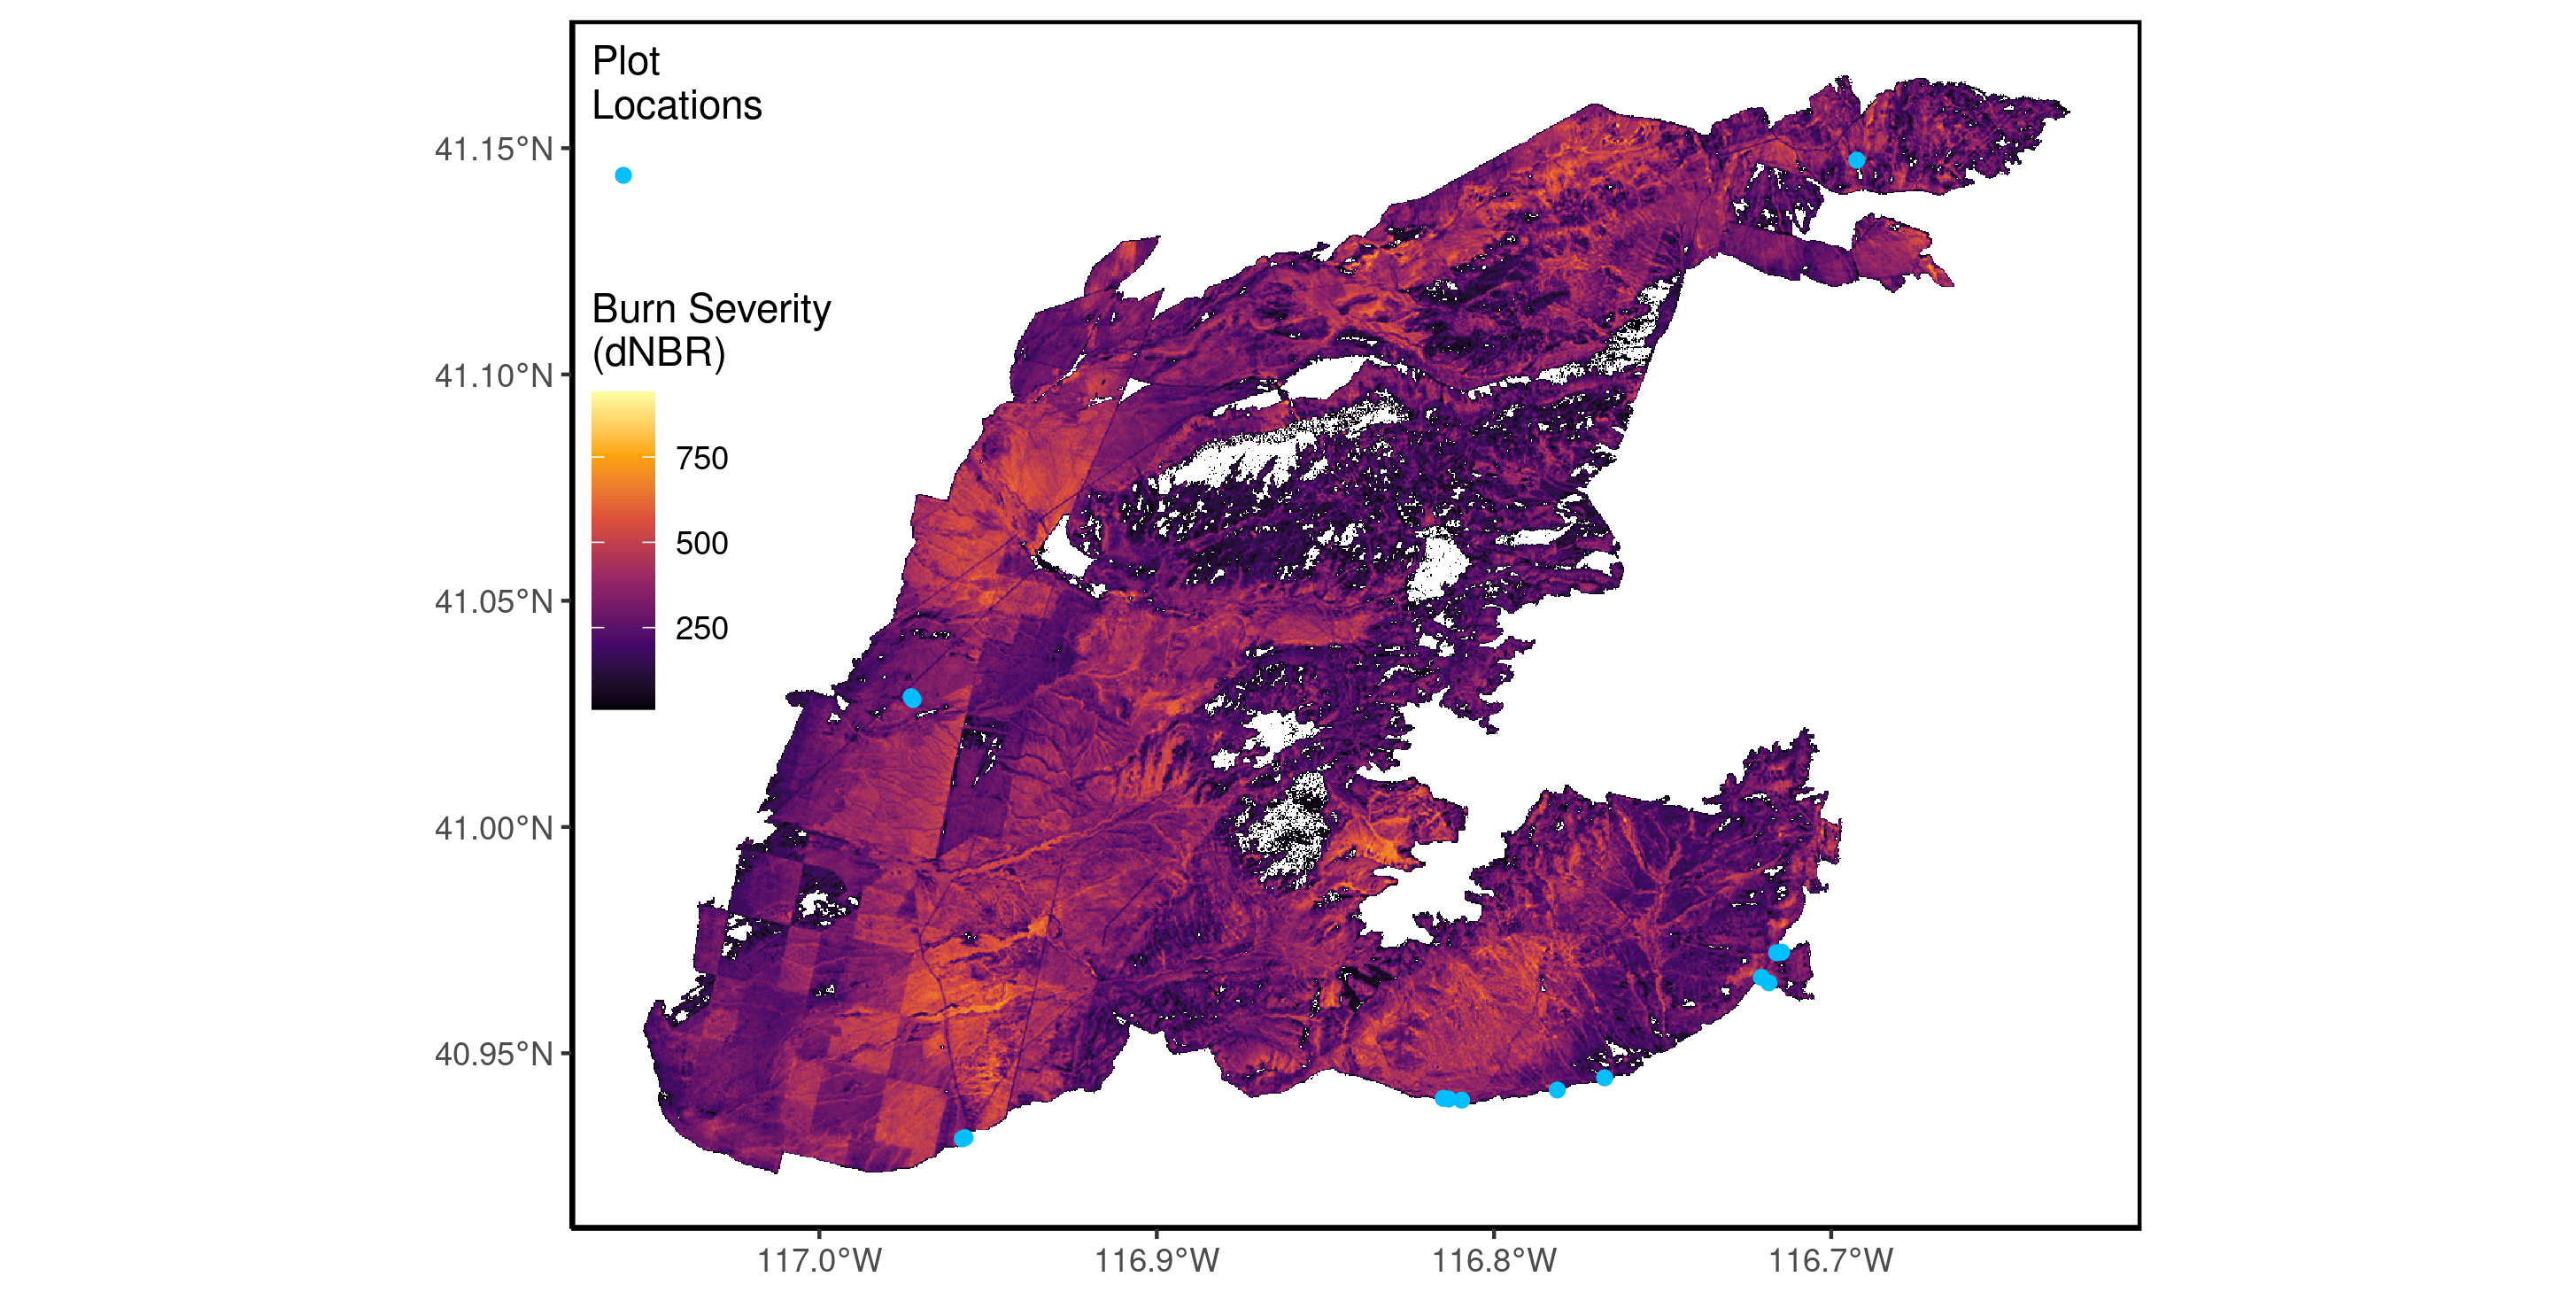
\includegraphics{images/map.png}
\caption{The 2016 Hot Pot Fire. Blue points represent sampling locations
and the shaded color is the burn severity. The checkerboard pattern on
the lower left corresponds to patterns of land ownership.}
\end{figure}

\emph{2.2 Seed Bank Sampling}

In early July 2016, we collected samples of the soil seed bank at
fourteen locations the day after the Hot Pot fire was contained. Each
site was located at the perimeter of the fire where it was clearly
delineated by a bulldozer line or in one case a narrow dirt road. Eleven
sites were mature sagebrush communities with no history of fire since at
least 1984. Three plots had previously burned in 1984 according to the
Monitoring Trends in Burn Severity (MTBS) fire history
(\protect\hyperlink{ref-Eidenshink2007}{Eidenshink et al. 2007}) and had
high cover of \emph{B. tectorum}, but still had scattered sagebrush
cover. We used a metal stake to mark paired burned and unburned sampling
locations on each side of the perimeter, 10 m from the nearest evidence
of anthropogenic disturbance (i.e.~bulldozer effects, footprints)
associated with active fire suppression along the perimeter. Within 3 m
of each marker, we extracted 12, 6 cm deep, 5 cm diameter, soil cores.
Seeds of sagebrush generally do not fall far (\textless30 m) from their
parent plants in this system
(\protect\hyperlink{ref-Shinneman2016}{Shinneman and McIlroy 2016}), and
so they are not uniformly distributed
(\protect\hyperlink{ref-Boudell2002}{Boudell, Link, and Johansen 2002}).
In addition, seeds from \emph{B. tectorum}
(\protect\hyperlink{ref-Young1975}{Young and Evans 1975}) and
\emph{Artemisia} have different germination rates based on the
micro-site they find themselves in (i.e.~under a shrub or in the bare
ground between shrubs, \protect\hyperlink{ref-Eckert1986}{Eckert et al.
1986}). To account for these potentially confounding effects, we placed
half of the core locations under shrubs, and half in shrub interspaces.
In the burned areas, it was obvious where shrubs had been located. Even
when they were completely incinerated, their imprint remained on the
soil surface (\protect\hyperlink{ref-Bechtold2007}{Bechtold and Inouye
2007}; \protect\hyperlink{ref-Germino2018}{Germino et al. 2018}). To
examine the effect of seed depth, we divided each soil core into 0-2 cm
and 2-6 cm depths. Litter was aggregated with the 0-2 cm samples.
Samples were then placed in cold storage (\textasciitilde2 deg C) for 3
months (\protect\hyperlink{ref-Meyer2013}{Meyer, Monsen, and Mcarthur
2013}). At all sites, to be sure that we were at a site where sagebrush
germination could occur we checked for first year germinants on the
unburned side (we found them at all sites), and to ensure that there
were no confounding effects of post-fire seed dispersal, we determined
whether or not the sagebrush were flowering (they were not flowering at
all sites), and recorded species occupancy for all aboveground plant
species.

We followed the methodology of Ter Heert et al.
(\protect\hyperlink{ref-Heerdt1996}{1996}) to germinate the seeds. Each
sample was run through 0.2 mm sieve, and spread in a 3-5 mm layer over
the top of 1 - 4 pots. These pots were filled 3 cm deep with potting
soil, topped by a thin layer of sand. Pots were watered as needed to
stay at field capacity. Every week emerging germinants were identified,
counted and removed. Most of the germination occurred within 6 weeks,
and after 8 weeks we ended the germination assay.

\emph{2.3 Post-Fire Vegetation Sampling}

We sampled the vegetative occupancy and cover in May 2017, the growing
season immediately after the fire and again in September 2019. At each
location, we established 50m transects starting at the boundary of the
burned and unburned sides of the perimeter, running perpendicular to the
fire perimeter, and marked the transect ends with rebar. We measured the
occupancy and abundance of all plant species by measuring cover of every
species in 0.1 m\(^2\) quadrats spaced every 5 m along each transect. We
used the line intercept method to measure shrub cover and herbaceous
plant cover along the transect. Both live and dead plants were included
in these measurements. Total vegetation cover (TVC) was defined as the
sum of herbaceous plant cover and shrub cover.

\emph{2.4 Estimating Burn Severity with Landsat 8 OLI}

We downloaded the ``fire bundle'' of the Hot Pot fire from www.mtbs.gov.
This included cloud-free Landsat 8 scenes collected before the Hot Pot
fire, and already calculated layers of the Differenced Normalized Burn
Ratio (dNBR, \protect\hyperlink{ref-Miller2009}{J. D. Miller et al.
2009}). Because our sites were generally within 10 meters of the burn
perimeter, The pixels directly intersecting the plot locations were
likely to be mixed pixels (i.e.~containing burned and unburned ground).
To minimize this effect, we extracted all the dNBR values within a 120
meter buffer of each seed bank plot for pixels whose centroids fell
inside of the fire perimeter and calculated the mean.

\emph{2.5 Statistical Analysis}

Our statistical analysis centered around trying to understand each
component of the positive feedback loop posited by the 4 hypotheses
described above. In order to understand how pre-fire fuel connectivity
influenced burn severity (H1), we used total vegetation cover (TVC) from
two separate data sources as a proxy for fuel connectivity, and created
separate linear models with TVC as the predictor variable and burn
severity (dNBR, \protect\hyperlink{ref-Miller2009}{J. D. Miller et al.
2009}) as the response variable. With the field data we collected, we
created an ordinary least squares (OLS) linear model with burn severity
as the dependent variable and TVC (defined as shrub cover plus
herbaceous plant cover from the unburned side of the paired plots),
elevation and aspect as independent variables.

We were concerned that because our data were collected at the edge of
the fire, the burn severity calculated at each point may have included
partially burned pixels. So, as a supplement, we examined the same
relationship by creating a model of TVC using Landsat Thematic Mapper
(TM) surface reflectance data using TVC from the Bureau of Land
Management's Assessment, Inventory and Monitoring dataset (AIM,
\protect\hyperlink{ref-AIM}{U.S. Department of Interior 2018}). The AIM
dataset contained 813 sampling locations within the Central Basin and
Range ecoregion (\protect\hyperlink{ref-CEC2006}{Commission for
Environmental Cooperation 2006}) that were visited by BLM field crews
between 2011 and 2015. They were mostly sampled once but there were some
repeats, for 1,117 total measurements. For each of these points, we
extracted the surface reflectance values of each Landsat band for the
sampling year near peak biomass using a cloud-free scene from May or
early June. Then, we used those surface reflectance values to calculate
various vegetation indexes (Table S1), including the Green Normalized
Differenced Vegetation Index (Green NDVI, Equation 1), and Normalized
Differenced Senesced Vegetation Index (NDSVI, Equation 2). We used these
indexes to create generalized linear model of TVC with a beta
distribution. For this and all linear models, we started with the
largest possible model and used backwards selection following the
methodology of \protect\hyperlink{ref-Zuur2009}{Zuur et al.}
(\protect\hyperlink{ref-Zuur2009}{2009}). We used the final reduced
model to create a layer of predicted TVC for the study area for the
pre-fire scene, and extracted both our predictions of TVC and dNBR of
the fire from 1000 regularly-spaced points within the fire perimeter.
Finally, to quantify the effect of TVC on burn severity, we created an
OLS linear model with our modeled TVC and its second-order polynomial as
predictor variables and burn severity as the response variable.

\textbf{Equation 1:} \(Green~NDVI = \frac{NIR - Green}{NIR + Green}\)

\textbf{Equation 2:} \(NDSVI = \frac{SWIR_1 - Red}{SWIR_1 + Red}\)

To examine how burn severity affected the community composition of the
seed bank (H2), we created a joint species distribution model (JSDM) in
a Bayesian framework (\protect\hyperlink{ref-HMSC}{Tikhonov et al.
2020}) for the occurrence of all species germinated from the seed bank
that were found at more than one location. We created four Markov Chain
Monte Carlo (MCMC) chains, each consisting of 150,000 iterations. We
discarded the first 50,000 iterations for each chain and then recorded
every 100th for a total of 1,000 posterior samples per chain, and 4,000
total. We assessed model convergence using the effective sample size and
the potential scale reduction factor
(\protect\hyperlink{ref-Gelman1992}{Gelman, Rubin, and others 1992}). We
used the model to predict the probability of occurrence of germinable
seeds of a given species along a gradient of burn severity. We included
burn severity, elevation, aspect, pre-fire seedbank diversity and soil
depth as independent variables.

To account for the possibility of H2a as a confounding factor, we
included the Shannon-Weaver diversity index
(\protect\hyperlink{ref-Shannon1949}{Shannon and Weaver 1949}) in the
paired, unburned seed bank samples as one of the predictor variables in
our JSDM. We also created OLS models with the unburned species richness
and Shannon-Weaver diversity index predicted by prefire fuel
connectivity, with the expectation that pre-fire fuel connectivity would
have had a negative effect on the prefire seedbank diversity. To examine
how community composition and burn severity then affected subsequent
fuel connectivity (H3), we created OLS models with fuel connectivity
three years post-fire as the dependent variable, and burn severity, seed
counts for \emph{B. tectorum}, \emph{P. secunda} and other species,
elevation, aspect, depth, and alpha diversity as independent variables.
To examine how the resulting fuel connectivity was related to
biodiversity (H4), we used the diversity data and connectivity data that
we collected in 2019 to create a Poisson GLM with number of species
encountered aboveground at each plot location as the dependent variable,
as well as an OLS linear model with the Shannon-Weaver index
(\protect\hyperlink{ref-Shannon1949}{Shannon and Weaver 1949}) as a
dependent variable. We used fuel connectivity, elevation, and aspect as
independent variables.

All analyses were done in R (\protect\hyperlink{ref-R}{R Core Team
2020}). Data and code to recreate the analysis is freely available at
\url{https://www.github.com/admahood/seed-bank} (DOI available after
acceptance).

\hypertarget{results}{%
\subsection{3. Results}\label{results}}

We found support for each hypothesized component of the positive
feedback loop. For H1, the most parsimonious model for our \emph{in
situ} observations had only TVC as the predictor, which had a weak
positive relationship with burn severity (\(\beta\) = 2.4, p = 0.083,
R\(^2\) = 0.27, Figure 2a, Table S3). For our remotely sensed analysis,
our most parsimonious model of TVC explained 35\% of the variation and
had Green NDVI, NDSVI and their interaction as predictors (Table S3).
Our model of dNBR using the predicted TVC within the fire perimeter as a
predictor of dNBR explained 42\% of the variation and the relationship
between TVC and burn severity was positive and significant (p
\textless\textless{} 0.01, Figure 2a, Table S3).

The vast majority of seeds that germinated in the greenhouse were the
two most common grass species, \emph{P secunda} and \emph{B. tectorum}
(Table S2). Eight forb species were found in more than one location, and
these 10 prevalent species are those that were used in our JSDM. Burned
plots had an average of 34 \(\pm\) 32 total seeds in the top 2 cm, and
12 \(\pm\) 14 in the bottom 4 cm. Unburned plots had an average of 299
\(\pm\) 170 in the top 2 cm and 59 \(\pm\) 29 in the bottom 4 cm (Figure
S1). For H2, the JSDM converged well (Gelman diagnostics all very close
to 1 and the effective sample size centered on 4,000, Figure S2a).
Elevation had the most significant effects on individual species (Figure
S2b) and explained the most variance on average (36\% Figure S2c). Burn
severity explained 23\% of the variance on average and was supported at
the 95\% level for 5 species (Figure S2b). For the introduced species,
the predictions along a gradient of burn severity were positive for
\emph{B. tectorum}, \emph{Sisymbrium altissimum} L. and \emph{Lepidium
perfoliatum} L., and negative for \emph{Ceratocephala testiculata} and
\emph{Alyssum desertorum} Stapf (Figure 2b). For native species, the
effect of burn severity on occurrence was positive for \emph{A.
tridentata}, neutral for \emph{P. secunda} and negative for the
remaining species (Figure 2b). Testing H2a revealed a positive
relationship between pre-fire aboveground species diversity and pre-fire
fuel connectivity, and so we felt it was reasonable to rule out pre-fire
fuel connectivity as a confounding factor for H2.

For H3, we found that, after accounting for elevation, pre-fire
aboveground richness, and the number of \emph{P. secunda} seeds, the
number of \emph{B. tectorum} seeds in the postfire seedbank was
positively associated with the fuel connectivity in 2019 (\(\beta\) =
0.54, p = 0.01, Adj R\(^2\) = 0.75,Figure 3c, Table S3). For H4 the most
parsimonious model (Adj R\(^2\) = 0.89, Table S3) had elevation, aspect,
fuel connectivity and an interaction between elevation and fuel
connectivity as predictors of aboveground Shannon-Weaver alpha
diversity. Fuel connectivity was negatively associated with
Shannon-Weaver diversity (\(\beta\) = -0.28, p=0.004, Figure 3d).

\begin{figure}
\centering
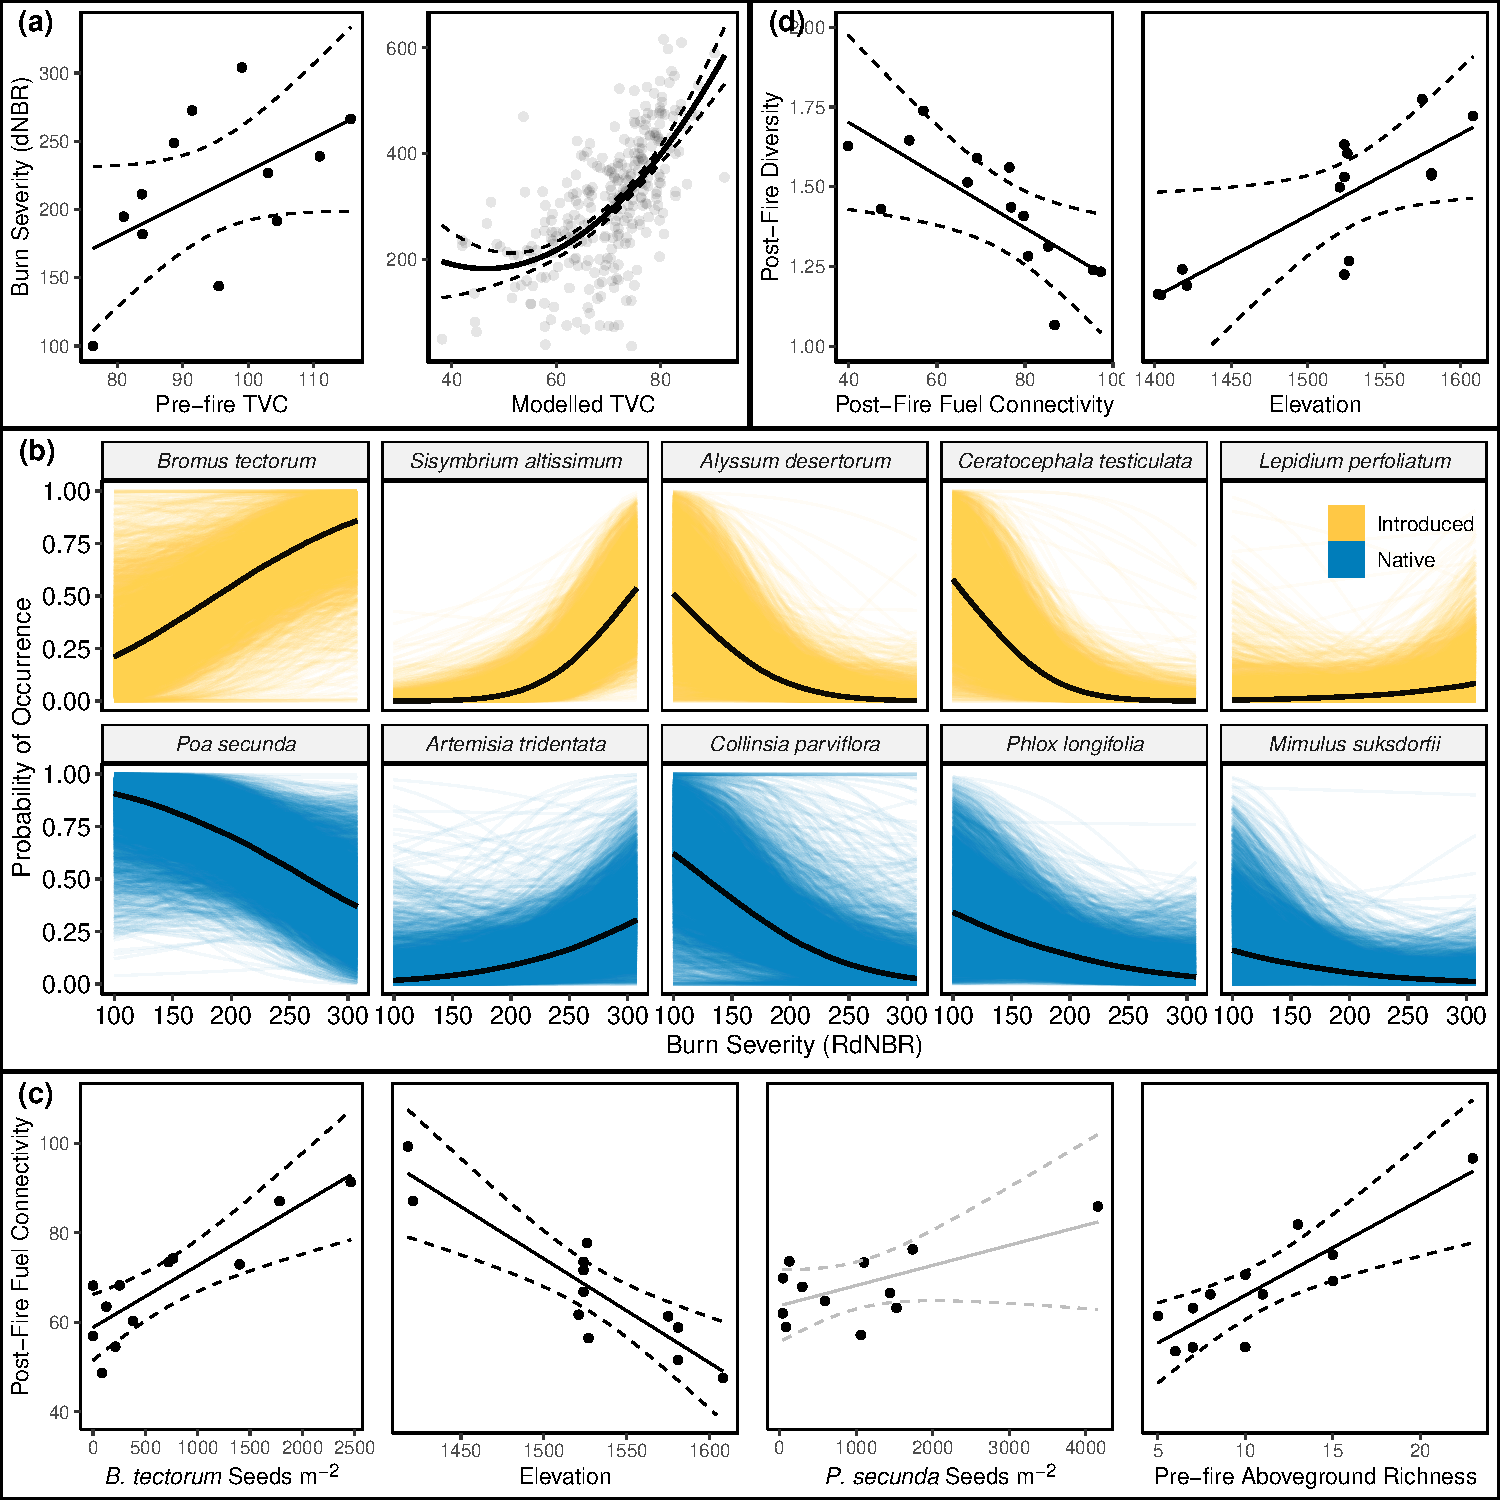
\includegraphics{images/big_plot.pdf}
\caption{On the left side of (a), burn severity (dNBR) as predicted by
total vegetation cover (TVC; the sum of live and dead, shrub and
herbaceous cover). On the right, burn severity is predicted by modelled
TVC. Panel b shows the modelled occurrence of germinable seeds for all
species found at more than one location along a gradient of burn
severity, after accounting for soil depth, aspect, elevation and
pre-fire diversity. Black line is the mean prediction, each colored line
represents one posterior sample. In (c), fuel connectivity three years
post-fire is modelled by seedbank composition, elevation and pre-fire
aboveground species richness. In (d) shannon-Weaver diversity index of
the aboveground, post-fire community composition, was negatively
affected by fuel connectivity after accounting for elevation. For a, c
and d, lines are the fitted partial effects, points are the partial
residuals, and dotted lines are the 95\% confidence intervals. p
\textless{} 0.05 for black lines, p \textgreater{} 0.05 for grey lines}
\end{figure}

\hypertarget{discussion}{%
\subsection{4. Discussion}\label{discussion}}

In order to truly consider an annual grass-fire cycle to be maintained
by self-reinforcing feedbacks, the mechanisms by which fire occurrence
is linked to higher post-fire flammability must be understood. In this
study we found that burn severity altered seed bank composition to favor
more flammable species. Prior work has shown that annual grass invasion
increases fuel connectivity in western US sagebrush ecosystems by
filling in shrub interspaces with a contiguous bed of fine fuels
(\protect\hyperlink{ref-Davies2013}{Davies and Nafus 2013}). This change
in the spatial distribution of fine fuels has been associated with
larger and more frequent fires (\protect\hyperlink{ref-Balch2013}{Balch
et al. 2013}). Here, we found higher fuel connectivity (via TVC) also
increases burn severity (H1, Figure 2a). Higher burn severity was
associated with an increased occurrence of introduced annuals in the
seedbank and a decreased occurrence of native plants (H2, Figure 2b).
Higher abundance of \emph{B. tectorum} seeds in the post-fire seedbank
resulted in higher post-fire fuel connectivity (H3, Figure 2c). In
addition, we found evidence that high post-fire fuel connectivity was
associated with lower aboveground diversity (H4, Figure 2d). This
suggests that during inter-fire intervals, there may be additional
mechanisms (e.g.~competition) maintaining the post-fire, annual
grass-dominated species assemblage.

The difference in species composition before and after fire explains an
apparent contradiction in results between H2a (positive relationship
between pre-fire fuel connectivity and diversity) and H4 (negative
relationship between post-fire fuel connectivity and diversity). Most
plot locations had mature canopies of native shrubs and with the
inter-shrub space occupied mostly by native bunchgrasses and forbs, with
no fire occurrence since 1984. Even in locations with high annual grass
cover between shrubs, shrubs provide ecosystem structural heterogeneity
and islands of fertility (\protect\hyperlink{ref-Doescher1984}{Doescher,
Miller, and Winward 1984}; \protect\hyperlink{ref-Bechtold2007}{Bechtold
and Inouye 2007}), and perennial natives that may have been established
before invasion have deep roots established that allow for the avoidance
of competition for water with shallow-rooted annuals
(\protect\hyperlink{ref-Gibbens2001}{Gibbens and Lenz 2001};
\protect\hyperlink{ref-Ottaviani2020}{Ottaviani et al. 2020}). This may
provide enough niche compartmentalization to allow native plants to
persist. Three years after the Hot Pot fire, almost all of the plots
were dominated by introduced annuals, and lacked any structural
heterogeneity. Thus native plants may have been be able to persist via
niche compartmentalization after the initial invasion, but fire burns
away most of the seeds (Figure S1) and removes all of the structural
benefits that shrub cover provides. In this clean slate post-fire
environment, the altered species composition of the seedbank and
superior post-fire dispersal of \emph{B. tectorum}
(\protect\hyperlink{ref-Monty2013}{Monty, Brown, and Johnston 2013})
allows the process of interspecific competition to be dominant
(\protect\hyperlink{ref-Schlaepfer2014}{Schlaepfer, Lauenroth, and
Bradford 2014}).

\emph{Global impacts}

The grass-fire cycle in the western US is reinforced through providing
fitness benefits to the introduced annual grasses and forbs via at least
4 redundant processes: i) changing the composition of the seedbank, ii)
competitive exclusion of native plants, iii) CO\(_2\) enrichment which
may preferentially enhance biomass (i.e.~higher fuel connectivity) and
seed production of annual grass species
(\protect\hyperlink{ref-Nagel2004}{Nagel et al. 2004};
\protect\hyperlink{ref-Smith2000}{Smith et al. 2000}), strengthening the
fuel connectivity to burn severity to seed composition feedback loop,
and iv) ecohydrological feedbacks that create a warmer, drier
microclimate (\protect\hyperlink{ref-Turnbull2012}{Turnbull et al.
2012}; \protect\hyperlink{ref-Wilcox2012}{Wilcox et al. 2012}). It is
likely that some of these feedbacks are idiosyncratic to the system
being studied, while others may reflect the fundamental properties of
ecosystem function that change when a system is converted from being
dominated by woody plants to being dominated by herbaceous plants
(\protect\hyperlink{ref-Kitzberger2016}{Kitzberger et al. 2016}).
Understanding the mechanisms of hysteresis, and in particular how
multiple redundant mechanisms act in concert, will provide important
insights for ecosystem change on a global scale. At least 13 grass
species initiate self-reinforcing feedbacks with fire in the U.S.
(\protect\hyperlink{ref-Fusco2019}{Fusco et al. 2019};
\protect\hyperlink{ref-Tortorelli2020}{Tortorelli, Krawchuk, and Kerns
2020}), and many more worldwide, including Australia
(\protect\hyperlink{ref-Miller2010}{G. Miller et al. 2010};
\protect\hyperlink{ref-Setterfield2010}{Setterfield et al. 2010}),
Brazil (\protect\hyperlink{ref-Rossi2014}{Rossi et al. 2014}) and South
Africa (\protect\hyperlink{ref-Milton2004}{Milton 2004}). While the
conversion of temperate forests and shrublands to grasslands may have a
less per-hectare impact on carbon sequestration than tropical forests,
the consequences are still relevant to the global carbon cycle,
especially when forests (rather than the shrublands studied here) are
replaced by herbaceous ecosystems
(\protect\hyperlink{ref-Kerns2020}{Kerns et al. 2020}).

\emph{Potential limitations}

We found fewer species and lower diversity in our seedbank germination
assays than we did in the aboveground sampling (Figure S3). This result
may be influenced by the methodological limitations inherent to
greenhouse germination trials
(\protect\hyperlink{ref-Vandvik2016}{Vandvik et al. 2016}). In
particular our results may be understating the occurrence of native
species in the seedbank. Habitat specialists have been shown to emerge
more in \emph{in situ} germination assays than in greenhouse germination
assays, while the opposite has been found for ruderal species
(\protect\hyperlink{ref-Plue2017}{Plue et al. 2017}). Nevertheless, for
those species that were prevalent in our germination studies, we still
found consistent relationships between their abundance and occurrence by
biogeographic origin, and those species that were prevalent in the
postfire seedbank germination assays were also those most common in the
aboveground community postfire.

\emph{Contrasts among forests and shrublands as it pertains to remote
sensing}

Burn severity metrics like dNBR were conceived of in the context of
forested ecosystems (\protect\hyperlink{ref-Miller2009}{J. D. Miller et
al. 2009}), and calibrated using the composite burn index
(\protect\hyperlink{ref-Key1999}{Key and Benson 1999}), tree mortality,
and percent change in tree canopy cover. These do not apply in shrubland
systems. Here we estimated burn severity using dNBR and understand it to
be a proxy for the amount of biomass that was burned in the fire. We
recorded qualitative observations of burn severity while we were
sampling, mainly to ensure that we sampled a range of severities, and
the dNBR we used appears to be a good proxy for our observations. The
Hot Pot fire took place during a high wind event, burning 50,000 ha in
only 3 days, so the scale of weather-driven fire spread overtook any
possibility of fuel disconnectivity on the scale of a few meters
stopping the spread of the fire. In areas where the space between shrubs
was well-connected by fine fuels (Figure 6a-c) the dNBR was higher, and
the shrubs had completely burned throughout the root system, leaving
only a hole in the ground filled with ashes as evidence of their prior
presence. In these areas the entirety of the soil surface---underneath
shrub canopy and in canopy interspaces---was consumed by fire, and there
was little evidence of remaining litter or biological soil crust. In
areas with lower fuel connectivity (Figure 6d-f), and lower dNBR, shrubs
were usually consumed only to the stumps, and sometimes were left
standing and charred, destined for mortality. In these areas the soil
surface often still had biological soil crust, partially consumed litter
(\protect\hyperlink{ref-Jones2015}{Jones et al. 2015}) and unconsumed
annual and perennial grass bases. We note that the manual severity
classification provided by MTBS had exclusively low and medium severity,
but our observations of essentially complete consumption of plant and
litter tissues and very few unburned patches suggested that these should
have been mostly medium and high severity. This discrepancy was not
unexpected, as the classified burn severity is known to be of limited
use for research (\protect\hyperlink{ref-Kolden2015}{Kolden, Smith, and
Abatzoglou 2015}).

Spectral reflectance has long been used to characterize wildfire fuels.
Unique signatures of remotely-sensed spectral reflectance are typically
matched to categorical fuel classifications (CFCs), which describe the
physiognomy of vegetation and its potential to support various fire
behavior (\protect\hyperlink{ref-Ottmar2007}{Ottmar et al. 2007}). While
different CFCs can provide a general understanding of fuel amount and
connectivity, recent efforts using data with finer spatial and spectral
resolution may improve fuel classification with more continuous,
multi-dimensional measurements
(\protect\hyperlink{ref-Stavros2018}{Stavros et al. 2018}). The
continuous measure of NDVI in western U.S. coniferous forests is a proxy
for live fuel biomass, which likely explains its positive association
with wildfire severity (\protect\hyperlink{ref-Parks2018}{Parks et al.
2018}; \protect\hyperlink{ref-Koontz2020}{Koontz et al. 2020}). NDVI
also correlates with vegetation cover in these forested systems, and so
greater crown connectivity may also explain the NDVI/severity
relationship at local scales. When using a more direct NDVI-derived
measure of vegetation connectivity in Sierra Nevada yellow
pine/mixed-conifer, \protect\hyperlink{ref-Koontz2020}{Koontz et al.}
(\protect\hyperlink{ref-Koontz2020}{2020}) found that greater
variability in forest structure also increased the probability of
high-severity fire. Here, we arrived at a combination of NDVI and NDSVI
to describe the fuel connectivity of the annual grass invaded Great
Basin sagebrush community to better reflect key differences in the
physiognomies of forest and arid shrublands. In sagebrush shrublands,
the fuel that contributes to large wildfires is a mixture of evergreen
shrubs interspersed with herbaceous plants that remain green for only a
portion of the growing season, and then become dry and straw-colored.
Thus, both the live and dead fuel need to be taken into account in
remote measurements of fuel connectivity.

\begin{figure}
\centering
\includegraphics[width=0.7\textwidth,height=\textheight]{images/burnsev_fig.pdf}
\caption{Visual illustration of the relationship between fuel
connectivity and burn severity. On the left, panel a shows the
intershrub space invaded by annual grasses. The photo in panel b was
taken in the exact same place two weeks later, days after all of the
biomass was consumed by the fire. Panel C is a closeup of the soil
surface, showing in more detail how the litter was also almost
completely consumed by the fire. On the right, the photos in panels d
and e were on opposite sides of a fire line in an area that had minimal
annual grass invasion over a broad area, and thus lower fuel
connectivity. Note the remaining plants and stumps in panel e and the
presence of only partially consumed litter in panel f.}
\end{figure}

\emph{Management implications}

These results demonstrate that the strength of the grass-fire cycle in
this system is controlled by measurable fire properties and ecosystem
structural components. Land managers may be able to increase their
chances of restoration success by using existing methods or developing
novel ones that manipulate these components to weaken or even break the
positive feedback cycle. This work provides further evidence that the
post-fire annual grassland is a system where the degraded state
represents an alternative species assemblage from that of the
restoration target. Because the propagules of the original assemblage
are no longer present, methods that rely on natural succession may not
be sufficient (\protect\hyperlink{ref-Suding2004}{Suding, Gross, and
Houseman 2004}). Our results highlight the importance of prioritizing
the preservation of native shrub cover and in particular policies that
encourage land managers to maximize the preservation of unburned patches
during the suppression of wildfires in this system
(\protect\hyperlink{ref-Steenvoorden2019}{Steenvoorden et al. 2019}).
Commonly encountered native plants and the keystone shrub species
\emph{A. tridentata} depend on post-fire seed dispersal from surviving
individuals in unburned patches
(\protect\hyperlink{ref-Schlaepfer2014}{Schlaepfer, Lauenroth, and
Bradford 2014}). Once the system achieves a canopy dominated by annual
grasses and forbs, the competitive pressure from the annual grass
monoculture makes it more difficult if not impossible for perennial
native forbs and shrubs to establish from the depleted seedbank.
Post-fire seeding efforts may restore native propagules, but if there is
dense cover of annuals further effort may be required to reduce fuel
connectivity in order to reduce both fire risk and competitive pressure
from annuals. Our results also suggest that calculating the burn
severity using Landsat or Sentinel images may help land managers
identify areas with a greater likelihood of successful seeding.

Livestock grazing can reduce fuel connectivity in uninvaded sagebrush
(\protect\hyperlink{ref-Davies2010}{Davies et al. 2010}). At the same
time, livestock grazing can decrease the resistance to invasion by
\emph{B. tectorum} via negative effects on biological soil crust (BSC)
(\protect\hyperlink{ref-chambers_resilience_2014}{Chambers et al. 2014};
\protect\hyperlink{ref-Condon2018}{Condon and Pyke 2018}), and can
reduce the survival of \emph{Artemisia} seedlings that are not protected
by shrub canopies (\protect\hyperlink{ref-Owens1992}{Owens and Norton
1992}). In wet years, targeted grazing at already invaded sagebrush
sites may reduce fuel connectivity and alleviate fire risk. Plant
community composition in the years immediately after fire may be highly
variable spatially and from year to year. Post-fire grazing may help
reduce \emph{B. tectorum} cover, but it may also exacerbate the problem
by introducing cheatgrass in uninvaded sites
(\protect\hyperlink{ref-Williamson2019}{Williamson et al. 2019}) or
increasing the already superior postfire dispersal of \emph{B. tectorum}
seeds (\protect\hyperlink{ref-Monty2013}{Monty, Brown, and Johnston
2013}). We suggest management approaches that are specifically tailored
each year to the conditions of a given site, and targeting grazing only
in already invaded areas to reduce \emph{B. tectorum} cover where it may
aid in native plant restoration.

Greenhouse or \emph{in situ} germination assays are time-consuming and
require botanical expertise, and are very important. There are many
studies that only study fire occurrence as it relates to the seed bank.
One potential avenue for future research may be linking
satellite-derived estimates of burn severity
(\protect\hyperlink{ref-Parks2018}{Parks et al. 2018}) and TVC with
locations of prior studies in retrospective meta-analyses. Teasing out
these mechanisms will increase our understanding of how generalizable
these phenomena are, and may provide more insight on how to mediate the
negative effects or break the positive feedback loop.

\hypertarget{acknowledgements}{%
\subsection{Acknowledgements}\label{acknowledgements}}

We thank Abdelhakim Farid, Julia Lopez, Dylan Murphy and C. Nick
Whittemore for their help in the field and in the greenhouse. We also
appreciate the use of the University of Colorado Boulder's Ecology
Evolution and Biology Greenhouse. We thank Lindsay P. Chiquoine and
Thomas T. Veblen for constructive feedback that greatly improved the
manuscript. We are grateful to everyone in the Winnemucca office of the
Bureau of Land Management and the Central Nevada Interagency Dispatch
Center for their help in the field. This project was funded in part by
the CU Boulder Geography department's Adam Kolff Memorial Graduate
Research Grant and CU Boulder's Undergraduate Research Opportunities
Program.

\hypertarget{references}{%
\subsection{References}\label{references}}

\singlespacing

\hypertarget{refs}{}
\begin{CSLReferences}{1}{0}
\leavevmode\hypertarget{ref-Andersen2009}{}%
Andersen, Tom, Jacob Carstensen, Emilio Hernández-García, and Carlos M.
Duarte. 2009. {``{Ecological thresholds and regime shifts: approaches to
identification}.''} \emph{Trends in Ecology and Evolution} 24 (1):
49--57. \url{https://doi.org/10.1016/j.tree.2008.07.014}.

\leavevmode\hypertarget{ref-Baker2006}{}%
Baker, William L. 2006. {``{Fire and restoration of sagebrush
ecosystems}.''} \emph{Wildlife Society Bulletin} 34 (1): 177--85.
\url{https://doi.org/10.2193/0091-7648(2006)34\%5B177:farose\%5D2.0.co;2}.

\leavevmode\hypertarget{ref-Balch2013}{}%
Balch, Jennifer K., Bethany A. Bradley, Carla M. D'Antonio, and José
Gómez-Dans. 2013. {``{Introduced annual grass increases regional fire
activity across the arid western USA (1980-2009)}.''} \emph{Global
Change Biology} 19 (1): 173--83.
\url{https://doi.org/10.1111/gcb.12046}.

\leavevmode\hypertarget{ref-Barga2018}{}%
Barga, Sarah, and Elizabeth A. Leger. 2018. {``{Shrub cover and fire
history predict seed bank composition in Great Basin shrublands}.''}
\emph{Journal of Arid Environments} 154 (November 2017): 40--50.
\url{https://doi.org/10.1016/j.jaridenv.2018.03.004}.

\leavevmode\hypertarget{ref-Bechtold2007}{}%
Bechtold, H. A., and R. S. Inouye. 2007. {``{Distribution of carbon and
nitrogen in sagebrush steppe after six years of nitrogen addition and
shrub removal}.''} \emph{Journal of Arid Environments} 71 (1): 122--32.
\url{https://doi.org/10.1016/j.jaridenv.2007.02.004}.

\leavevmode\hypertarget{ref-Beckstead2011}{}%
Beckstead, Julie, Laura E. Street, Susan E. Meyer, and Phil S. Allen.
2011. {``{Fire effects on the cheatgrass seed bank pathogen Pyrenophora
semeniperda}.''} \emph{Rangeland Ecology and Management} 64 (2):
148--57. \url{https://doi.org/10.2111/REM-D-10-00052.1}.

\leavevmode\hypertarget{ref-Bond1995}{}%
Bond, William J., and Jeremy J. Midgley. 1995. {``{Kill Thy Neighbour:
An Individualistic Argument for the Evolution of Flammability}.''}
\emph{Oikos} 73 (1): 79. \url{https://doi.org/10.2307/3545728}.

\leavevmode\hypertarget{ref-Boudell2002}{}%
Boudell, JA, SO Link, and JR Johansen. 2002. {``{Effect of soil
microtopography on seed bank distribution in the shrub-steppe}.''}
\emph{Western North American Naturalist} 62 (1): 14--24.
\url{https://doi.org/10.2307/41717153}.

\leavevmode\hypertarget{ref-Bradford2020}{}%
Bradford, John B., Daniel R. Schlaepfer, William K. Lauenroth, and Kyle
A. Palmquist. 2020. {``{Robust ecological drought projections for
drylands in the 21st century}.''} \emph{Global Change Biology} 26 (7):
3906--19. \url{https://doi.org/10.1111/gcb.15075}.

\leavevmode\hypertarget{ref-Brooks2004}{}%
Brooks, Matthew L., Carla M. D'Antonio, David M. Richardson, James B.
Grace, Jon E. Keeley, Joseph M. DiTomaso, Richard J. Hobbs, Mike
Pellant, and David Pyke. 2004. {``{Effects of Invasive Alien Plants on
Fire Regimes}.''} \emph{BioScience} 54 (7): 677--88.

\leavevmode\hypertarget{ref-Bukowski2013}{}%
Bukowski, Beth, and William L. Baker. 2013. {``{Historical fire regimes,
reconstructed from land-survey data, led to complexity and fluctuation
in sagebrush landscapes}.''} \emph{Ecological Applications} 23 (3):
546--64.

\leavevmode\hypertarget{ref-chambers_resilience_2014}{}%
Chambers, Jeanne C., Bethany A. Bradley, Cynthia S. Brown, Carla M.
D'Antonio, Matthew J. Germino, James B. Grace, Stuart P. Hardegree,
Richard F. Miller, and David A. Pyke. 2014. {``Resilience to Stress and
Disturbance, and Resistance to {Bromus} Tectorum {L}. Invasion in Cold
Desert Shrublands of Western {North} {America}.''} \emph{Ecosystems} 17
(2): 360--75. \url{https://doi.org/10.1007/s10021-013-9725-5}.

\leavevmode\hypertarget{ref-Chambers2007}{}%
Chambers, Jeanne C., Bruce A. Roundy, Robert R. Blank, Susan E. Meyer,
and A. Whittaker. 2007. {``{What makes Great Basin sagebrush ecosystems
invasible by Bromus tectorum?}''} \emph{Ecological Monographs} 77 (1):
117--45. \url{https://doi.org/10.1890/05-1991}.

\leavevmode\hypertarget{ref-CEC2006}{}%
Commission for Environmental Cooperation. 2006. {``{Ecological regions
of North America -- Levels I, II, and III: Montreal, Quebec, Canada,
Commission for Environmental Cooperation, scale 1:10,000,000}.''}
\url{https://www.epa.gov/eco-research/ecoregions-north-america}.

\leavevmode\hypertarget{ref-Condon2018}{}%
Condon, Lea A., and David A. Pyke. 2018. {``{Fire and Grazing Influence
Site Resistance to Bromus tectorum Through Their Effects on Shrub,
Bunchgrass and Biocrust Communities in the Great Basin (USA)}.''}
\emph{Ecosystems} 21 (7): 1416--31.
\url{https://doi.org/10.1007/s10021-018-0230-8}.

\leavevmode\hypertarget{ref-DAntonio1992}{}%
D'Antonio, Carla M., and Peter M. Vitousek. 1992. {``{Biological
invasions by exotic grasses, the grass/fire cycle, and global
change}.''} \emph{Annual Review of Ecological Systems} 23: 63--87.

\leavevmode\hypertarget{ref-Davies2010}{}%
Davies, Kirk W., Jonathan D. Bates, Tony J. Svejcar, and Chad S. Boyd.
2010. {``{Effects of long-term livestock grazing on fuel characteristics
in rangelands: An example from the sagebrush steppe}.''} \emph{Rangeland
Ecology and Management} 63 (6): 662--69.
\url{https://doi.org/10.2111/REM-D-10-00006.1}.

\leavevmode\hypertarget{ref-Davies2011}{}%
Davies, Kirk W., Chad S. Boyd, Jeffrey L. Beck, Jon D. Bates, Tony J.
Svejcar, and Michael A. Gregg. 2011. {``{Saving the sagebrush sea: An
ecosystem conservation plan for big sagebrush plant communities}.''}
\emph{Biological Conservation} 144 (11): 2573--84.
\url{https://doi.org/10.1016/j.biocon.2011.07.016}.

\leavevmode\hypertarget{ref-Davies2013}{}%
Davies, Kirk W., and Aleta M. Nafus. 2013. {``{Exotic annual grass
invasion alters fuel amounts, continuity and moisture content}.''}
\emph{International Journal of Wildland Fire} 22 (3): 353--58.
\url{https://doi.org/10.1071/WF11161}.

\leavevmode\hypertarget{ref-Davis2000}{}%
Davis, Mark A., J P Grime, Ken Thompson, and J Philip. 2000.
{``{Fluctuating resources in plant communities: a general of
invasibility theory}.''} \emph{Journal of Ecology} 88 (3): 528--34.
\url{https://doi.org/10.1046/j.1365-2745.2000.00473.x}.

\leavevmode\hypertarget{ref-Doescher1984}{}%
Doescher, Paul S., Richard F. Miller, and Alma H. Winward. 1984.
{``{Soil Chemical Patterns under Eastern Oregon Plant Communities
Dominated by Big Sagebrush}.''}
\url{https://doi.org/10.2136/sssaj1984.03615995004800030038x}.

\leavevmode\hypertarget{ref-Eckert1986}{}%
Eckert, Richard E., Frederick F. Peterson, Michael S. Meurisse, and L.
Stephens. 1986. {``{Effects of Soil-Surface Morphology on Emergence and
Survival of Seedlings in Big Sagebrush Communities}.''} \emph{Journal of
Range Management} 39 (5): 414--20.
\url{http://www.jstor.org/stable/3899441}.

\leavevmode\hypertarget{ref-Eidenshink2007}{}%
Eidenshink, Jeff, Brian Schwind, Ken Brewer, Zhi-liang Zhu, Brad Quayle,
and Stephen Howard. 2007. {``{A Project for Monitoring Trends in Burn
Severity}.''} \emph{Fire Ecology} 3 (1): 3--21.
\url{https://doi.org/10.4996/fireecology.0301003}.

\leavevmode\hypertarget{ref-Fusco2019}{}%
Fusco, Emily J., John T. Finn, Jennifer K. Balch, R. Chelsea Nagy, and
Bethany A. Bradley. 2019. {``Invasive Grasses Increase Fire Occurrence
and Frequency Across US Ecoregions.''} \emph{Proceedings of the National
Academy of Sciences} 116 (47): 23594--99.
\url{https://doi.org/10.1073/pnas.1908253116}.

\leavevmode\hypertarget{ref-Gagnon2015}{}%
Gagnon, Paul R., Heather A. Passmore, Matthew Slocum, Jonathan A. Myers,
Kyle E. Harms, William J. Platt, and C. E. Timothy Paine. 2015.
{``{Fuels and fires influence vegetation via above- and belowground
pathways in a high-diversity plant community}.''} \emph{Journal of
Ecology} 103 (4): 1009--19.
\url{https://doi.org/10.1111/1365-2745.12421}.

\leavevmode\hypertarget{ref-Gelman1992}{}%
Gelman, Andrew, Donald B Rubin, and others. 1992. {``Inference from
Iterative Simulation Using Multiple Sequences.''} \emph{Statistical
Science} 7 (4): 457--72.

\leavevmode\hypertarget{ref-Germino2018}{}%
Germino, Matthew J., David M. Barnard, Bill E. Davidson, Robert S.
Arkle, David S. Pilliod, Matthew R. Fisk, and Cara Applestein. 2018.
{``{Thresholds and hotspots for shrub restoration following a
heterogeneous megafire}.''} \emph{Landscape Ecology} 33 (7): 1177--94.
\url{https://doi.org/10.1007/s10980-018-0662-8}.

\leavevmode\hypertarget{ref-Germino2016}{}%
Germino, Matthew J., Jeanne C. Chambers, and Cynthia S. Brown. 2016.
\emph{{Exotic Brome-Grasses in Arid and Semiarid Ecosystems of the
Western US Causes, Consequences, and Management Implications}}.
\url{http://www.springer.com/series/412}.

\leavevmode\hypertarget{ref-Gibbens2001}{}%
Gibbens, Robert P., and James M. Lenz. 2001. {``{Root systems of some
Chihuahuan Desert plants}.''} \emph{Journal of Arid Environments} 49:
221--63.

\leavevmode\hypertarget{ref-Hassan1986}{}%
Hassan, M. A., and N. E. West. 1986. {``{Dynamics of Soil Seed Pools in
Burned and Unburned Sagebrush Semi-Deserts}.''} \emph{Ecology} 67 (1):
269--72.

\leavevmode\hypertarget{ref-Heerdt1996}{}%
Heerdt, G. N. J. Ter, G. L. Verweij, R. M. Bekker, and J. P. Bakker.
1996. {``{An Improved Method for Seed-Bank Analysis: Seedling Emergence
After Removing the Soil by Sieving}.''} \emph{Functional Ecology} 10
(1): 144. \url{https://doi.org/10.2307/2390273}.

\leavevmode\hypertarget{ref-Heydari2017}{}%
Heydari, Mehdi, Reza Omidipour, Mehdi Abedi, and Carol Baskin. 2017.
{``{Effects of fire disturbance on alpha and beta diversity and on beta
diversity components of soil seed banks and aboveground vegetation}.''}
\emph{Plant Ecology and Evolution} 150 (3): 247--56.
\url{https://doi.org/10.5091/plecevo.2017.1344}.

\leavevmode\hypertarget{ref-Hirota2011}{}%
Hirota, Marina, Milena Holmgren, Egbert H. Van Nes, and Marten Scheffer.
2011. {``{Global resilience of tropical forest and savanna to critical
transitions}.''} \emph{Science} 334 (6053): 232--35.
\url{https://doi.org/10.1126/science.1210657}.

\leavevmode\hypertarget{ref-Humphrey2001}{}%
Humphrey, L David, and Eugene W Schupp. 2001. {``{Seed banks of Bromus
tectorum-dominated communities in the Great Basin}.''} \emph{Western
North American Naturalist} 61 (1): 85--92.
\url{https://doi.org/10.2307/41717080}.

\leavevmode\hypertarget{ref-Jones2015}{}%
Jones, Rachel O., Jeanne C. Chambers, David I. Board, Dale W. Johnson,
and Robert R. Blank. 2015. {``{The role of resource limitation in
restoration of sagebrush ecosystems dominated by cheatgrass (Bromus
tectorum)}.''} \emph{Ecosphere} 6 (7): 1--21.

\leavevmode\hypertarget{ref-Keeley2009}{}%
Keeley, Jon E. 2009. {``{Fire intensity, fire severity and burn
severity: A brief review and suggested usage}.''} \emph{International
Journal of Wildland Fire} 18 (1): 116--26.
\url{https://doi.org/10.1071/WF07049}.

\leavevmode\hypertarget{ref-Keeley2019}{}%
Keeley, Jon E., and Juli G. Pausas. 2019. {``{Distinguishing disturbance
from perturbations in fire-prone ecosystems}.''} \emph{International
Journal of Wildland Fire} 28 (4): 282--87.
\url{https://doi.org/10.1071/WF18203}.

\leavevmode\hypertarget{ref-Keeley2011}{}%
Keeley, Jon E., Juli G. Pausas, Philip W. Rundel, William J. Bond, and
Ross A. Bradstock. 2011. {``{Fire as an evolutionary pressure shaping
plant traits}.''} \emph{Trends in Plant Science} 16 (8): 406--11.
\url{https://doi.org/10.1016/j.tplants.2011.04.002}.

\leavevmode\hypertarget{ref-Kerns2020}{}%
Kerns, Becky K., Claire Tortorelli, Michelle A. Day, Ty Nietupski, Ana
M. G. Barros, John B. Kim, and Meg A. Krawchuk. 2020. {``{Invasive
grasses: A new perfect storm for forested ecosystems?}''} \emph{Forest
Ecology and Management} 463 (November 2019): 117985.
\url{https://doi.org/10.1016/j.foreco.2020.117985}.

\leavevmode\hypertarget{ref-Key1999}{}%
Key, Carl H, and Nathan C Benson. 1999. {``The Composite Burn Index
(CBI): Field Rating of Burn Severity.''} \emph{USGS, NRMSC
Research,{[}online{]} Available: Http://Nrmsc. Usgs. Gov/Research/Cbi.
Htm {[}3/14/2006{]}}.

\leavevmode\hypertarget{ref-Kimura2011}{}%
Kimura, Hideo, and Shiro Tsuyuzaki. 2011. {``{Fire severity affects
vegetation and seed bank in a wetland}.''} \emph{Applied Vegetation
Science} 14 (3): 350--57.
\url{https://doi.org/10.1111/j.1654-109X.2011.01126.x}.

\leavevmode\hypertarget{ref-Kitzberger2016}{}%
Kitzberger, Thomas, G. L. W. Perry, J. Paritsis, J. H. Gowda, A. J.
Tepley, A. Holz, and T. T. Veblen. 2016. {``{Fire--vegetation feedbacks
and alternative states: common mechanisms of temperate forest
vulnerability to fire in southern South America and New Zealand}.''}
\emph{New Zealand Journal of Botany} 54 (2): 247--72.
\url{https://doi.org/10.1080/0028825X.2016.1151903}.

\leavevmode\hypertarget{ref-Knapp1996}{}%
Knapp, Paul A. 1996. {``{Cheatgrass (Bromus tectorum L) dominance in the
Great Basin Desert}.''} \emph{Global Environmental Change} 6 (1):
37--52. \url{https://doi.org/10.1016/0959-3780(95)00112-3}.

\leavevmode\hypertarget{ref-Kolden2015}{}%
Kolden, Crystal A, Alistair M S Smith, and John T. Abatzoglou. 2015.
{``{Limitations and utilisation of Monitoring Trends in Burn Severity
products for assessing wildfire severity in the USA}.''}
\emph{International Journal of Wildland Fire} 24: 1023--28.

\leavevmode\hypertarget{ref-Koontz2020}{}%
Koontz, Michael J, Malcolm P North, Chhaya M Werner, Stephen E Fick, and
Andrew M Latimer. 2020. {``Local Forest Structure Variability Increases
Resilience to Wildfire in Dry Western US Coniferous Forests.''}
\emph{Ecology Letters} 23 (3): 483--94.

\leavevmode\hypertarget{ref-Lipoma2018}{}%
Lipoma, M. Lucrecia, Guillermo Funes, and Sandra Díaz. 2018. {``{Fire
effects on the soil seed bank and post-fire resilience of a semi-arid
shrubland in central Argentina}.''} \emph{Austral Ecology} 43 (1):
46--55. \url{https://doi.org/10.1111/aec.12533}.

\leavevmode\hypertarget{ref-Liyanage2017}{}%
Liyanage, Ganesha S., and Mark K. J. Ooi. 2017. {``{Do dormancy-breaking
temperature thresholds change as seeds age in the soil seed bank?}''}
\emph{Seed Science Research} 27 (1): 1--11.
\url{https://doi.org/10.1017/S0960258516000271}.

\leavevmode\hypertarget{ref-Mahood2019}{}%
Mahood, Adam L., and Jennifer K. Balch. 2019. {``{Repeated fires reduce
plant diversity in low-elevation Wyoming big sagebrush ecosystems (1984
-- 2014)}.''} \emph{Ecosphere} 10 (2): e02591.
\url{https://doi.org/10.1002/ecs2.2591}.

\leavevmode\hypertarget{ref-Maia2012}{}%
Maia, P., J. G. Pausas, V. Arcenegui, C. Guerrero, A. Pérez-Bejarano, J.
Mataix-Solera, M. E. T. Varela, I. Fernandes, E. T. Pedrosa, and J. J.
Keizer. 2012. {``{Wildfire effects on the soil seed bank of a maritime
pine stand - The importance of fire severity}.''} \emph{Geoderma} 191:
80--88. \url{https://doi.org/10.1016/j.geoderma.2012.02.001}.

\leavevmode\hypertarget{ref-Melillo2014}{}%
Melillo, Jerry M., Terese (T.C.) Richmond, and Gary W. Yohe. 2014.
\emph{Climate {Change} {Impacts} in the {United} {States}: {The} {Third}
{National} {Climate} {Assessment}. {U}.{S}.} U.S. Global Change Research
Program. \url{https://doi.org/10.7930/j0z31WJ2}.

\leavevmode\hypertarget{ref-Meyer1994}{}%
Meyer, Susan E. 1994. {``{Germination and establishment ecology of big
sagebrush: implications for community restoration}.''} In
\emph{Symposium on Management, Ecology, and Restoration of Lntermountain
Annual Rangelands, Boise, ID, May 18-21, 1992}, 244--51.

\leavevmode\hypertarget{ref-Meyer2013}{}%
Meyer, Susan E, Stephen B Monsen, and E Durant Mcarthur. 2013.
{``{Germination Response of Artemisia tridentata (Asteraceae) to Light
and Chill: Patterns of Between-Population Variation}.''} \emph{Botanical
Gazette} 151 (2): 176--83.

\leavevmode\hypertarget{ref-Miller2010}{}%
Miller, Georgia, Margaret Friedel, Paul Adam, and Vanessa Chewings.
2010. {``{Ecological impacts of buffel grass (Cenchrus ciliaris L.)
invasion in central Australia does field evidence support a
fire-invasion feedback?}''} \emph{The Rangeland Journal} 32 (4):
353--65. \url{https://doi.org/10.1071/RJ09076}.

\leavevmode\hypertarget{ref-Miller2009}{}%
Miller, Jay D., Eric E. Knapp, Carl H. Key, Carl N. Skinner, Clint J.
Isbell, R. Max Creasy, and Joseph W. Sherlock. 2009. {``{Calibration and
validation of the relative differenced Normalized Burn Ratio (RdNBR) to
three measures of fire severity in the Sierra Nevada and Klamath
Mountains, California, USA}.''} \emph{Remote Sensing of Environment} 113
(3): 645--56. \url{https://doi.org/10.1016/j.rse.2008.11.009}.

\leavevmode\hypertarget{ref-Milton2004}{}%
Milton, Sue J. 2004. {``{Grasses as invasive alien plants in South
Africa}.''} \emph{South African Journal of Science} 100 (1-2): 69--75.

\leavevmode\hypertarget{ref-Monty2013}{}%
Monty, Arnaud, Cynthia S. Brown, and Danielle B. Johnston. 2013.
{``{Fire promotes downy brome (Bromus tectorum L.) seed dispersal}.''}
\emph{Biological Invasions} 15 (5): 1113--23.
\url{https://doi.org/10.1007/s10530-012-0355-1}.

\leavevmode\hypertarget{ref-Morgan1988}{}%
Morgan, P., and L. F. Neuenschwander. 1988. {``Seed-Bank Contributions
to Regeneration of Shrub Species After Clear-Cutting and Burning.''}
\emph{Canadian Journal of Botany} 66 (1): 169--72.
\url{https://doi.org/10.1139/b88-026}.

\leavevmode\hypertarget{ref-Nagel2004}{}%
Nagel, Jennifer M., Travis E. Huxman, Kevin L. Griffin, and Stanley D.
Smith. 2004. {``{CO2 enrichment reduces the energetic cost of biomass
construction in an invasive desert grass}.''} \emph{Ecology} 85 (1):
100--106. \url{https://doi.org/10.1890/02-3005}.

\leavevmode\hypertarget{ref-Ottaviani2020}{}%
Ottaviani, Gianluigi, Rafael Molina-Venegas, Tristan Charles-Dominique,
Stefano Chelli, Giandiego Campetella, Roberto Canullo, and Jitka
Klimešová. 2020. {``{The Neglected Belowground Dimension of Plant
Dominance}.''} \emph{Trends in Ecology and Evolution} 35 (9): 763--66.
\url{https://doi.org/10.1016/j.tree.2020.06.006}.

\leavevmode\hypertarget{ref-Ottmar2007}{}%
Ottmar, Roger D, David V Sandberg, Cynthia L Riccardi, and Susan J
Prichard. 2007. {``An Overview of the Fuel Characteristic Classification
System---Quantifying, Classifying, and Creating Fuelbeds for Resource
Planning.''} \emph{Canadian Journal of Forest Research} 37 (12):
2383--93.

\leavevmode\hypertarget{ref-Owens1992}{}%
Owens, M. K., and B. E. Norton. 1992. {``{Interactions of Grazing and
Plant Protection on Basin Big Sagebrush (Artemisia tridentata ssp .
tridentata) Seedling Survival}.''} \emph{Journal of Range Management} 45
(3): 257--62. \url{http://www.jstor.org/stable/4002974}.

\leavevmode\hypertarget{ref-Palmer2018}{}%
Palmer, Harrison D., Andrew J. Denham, and Mark K. J. Ooi. 2018.
{``{Fire severity drives variation in post-fire recruitment and residual
seed bank size of Acacia species}.''} \emph{Plant Ecology} 219 (5):
527--37. \url{https://doi.org/10.1007/s11258-018-0815-5}.

\leavevmode\hypertarget{ref-Parks2018}{}%
Parks, Sean A., Lisa M. Holsinger, Morgan A. Voss, Rachel A. Loehman,
and Nathaniel P. Robinson. 2018. {``{Mean composite fire severity
metrics computed with google earth engine offer improved accuracy and
expanded mapping potential}.''} \emph{Remote Sensing} 10 (6): 1--15.
\url{https://doi.org/10.3390/rs10060879}.

\leavevmode\hypertarget{ref-Perryman2001}{}%
Perryman, Barry L, Aaron M Maier, Ann L Hild, and Richard A Olson. 2001.
{``{Demographic characteristics of 3 Artemisia tridentata Nutt.
subspecies}.''} \emph{Journal of Range Management} 54 (2): 166--70.

\leavevmode\hypertarget{ref-Petraitis1999}{}%
Petraitis, Peter S., and Roger Earl Latham. 1999. {``{The importance of
scale in testing the origins of alternative community states}.''}
\emph{Ecology} 80 (2): 429--42.
\url{https://doi.org/10.1890/0012-9658(1999)080\%5B0429:TIOSIT\%5D2.0.CO;2}.

\leavevmode\hypertarget{ref-Plue2017}{}%
Plue, J., F. Colas, A. G. Auffret, and S. A. O. Cousins. 2017.
{``{Methodological bias in the seed bank flora holds significant
implications for understanding seed bank community functions}.''}
\emph{Plant Biology} 19 (2): 201--10.
\url{https://doi.org/10.1111/plb.12516}.

\leavevmode\hypertarget{ref-R}{}%
R Core Team. 2020. \emph{R: A Language and Environment for Statistical
Computing}. Vienna, Austria: R Foundation for Statistical Computing.
\url{https://www.R-project.org/}.

\leavevmode\hypertarget{ref-Ratajczak2018}{}%
Ratajczak, Zak, Stephen R. Carpenter, Anthony R. Ives, Christopher J.
Kucharik, Tanjona Ramiadantsoa, M. Allison Stegner, John W. Williams,
Jien Zhang, and Monica G. Turner. 2018. {``{Abrupt Change in Ecological
Systems: Inference and Diagnosis}.''} \emph{Trends in Ecology and
Evolution} 33 (7): 513--26.
\url{https://doi.org/10.1016/j.tree.2018.04.013}.

\leavevmode\hypertarget{ref-Rossi2014}{}%
Rossi, Rafael Drumond, Carlos Romero Martins, Pedro Lage Viana, Evandro
Luís Rodrigues, and José Eugênio Côrtes Figueira. 2014. {``{Impact of
invasion by molasses grass (Melinis minutiflora P. Beauv.) on native
species and on fires in areas of campo-cerrado in Brazil}.''} \emph{Acta
Botanica Brasilica} 28 (4): 631--37.
\url{https://doi.org/10.1590/0102-33062014abb3390}.

\leavevmode\hypertarget{ref-Schimmel1996}{}%
Schimmel, Johnny, and Anders Granström. 1996. {``{Fire Severity and
Vegetation Response in the Boreal Swedish Forest}.''} \emph{Ecology} 77
(5): 1436--50.

\leavevmode\hypertarget{ref-Schlaepfer2014}{}%
Schlaepfer, Daniel R., William K. Lauenroth, and John B. Bradford. 2014.
{``{Natural Regeneration Processes in Big Sagebrush (Artemisia
tridentata)}.''} \emph{Rangeland Ecology \& Management} 67 (4): 344--57.
\url{https://doi.org/10.2111/REM-D-13-00079.1}.

\leavevmode\hypertarget{ref-Schwilk2002}{}%
Schwilk, Dylan W., and Benjamin Kerr. 2002. {``{Genetic niche-hiking: An
alternative explanation for the evolution of flammability}.''}
\emph{Oikos} 99 (3): 431--42.
\url{https://doi.org/10.1034/j.1600-0706.2002.11730.x}.

\leavevmode\hypertarget{ref-Setterfield2010}{}%
Setterfield, Samantha A., Natalie A. Rossiter-Rachor, Lindsay B. Hutley,
Michael M. Douglas, and Richard J. Williams. 2010. {``{Turning up the
heat: The impacts of Andropogon gayanus (gamba grass) invasion on fire
behaviour in northern Australian savannas}.''} \emph{Diversity and
Distributions} 16 (5): 854--61.
\url{https://doi.org/10.1111/j.1472-4642.2010.00688.x}.

\leavevmode\hypertarget{ref-Shannon1949}{}%
Shannon, CE, and W Weaver. 1949. {``The Mathematical Theory of
Communication. University of Illinois Press, Urbana-Champaign, Illinois,
USA, 117 p.''}

\leavevmode\hypertarget{ref-Shinneman2016}{}%
Shinneman, Douglas J., and Susan K. McIlroy. 2016. {``{Identifying key
climate and environmental factors affecting rates of post-fire big
sagebrush (Artemisia tridentata) recovery in the northern Columbia
Basin, USA}.''} \emph{International Journal of Wildland Fire} 25:
933--45. \url{https://doi.org/10.1071/WF16013}.

\leavevmode\hypertarget{ref-Shriver2018}{}%
Shriver, Robert K., Caitlin M. Andrews, David S. Pilliod, Robert S.
Arkle, Justin L. Welty, Matthew J. Germino, Michael C. Duniway, David A.
Pyke, and John B. Bradford. 2018. {``Adapting Management to a Changing
World: {Warm} Temperatures, Dry Soil, and Interannual Variability Limit
Restoration Success of a Dominant Woody Shrub in Temperate Drylands.''}
\emph{Global Change Biology} 24 (10): 4972--82.
\url{https://doi.org/10.1111/gcb.14374}.

\leavevmode\hypertarget{ref-Smith2000}{}%
Smith, Stanley D., Travis E. Huxman, Stephen F. Zitzer, Therese N.
Charlet, David C. Housman, James S. Coleman, Lynn K. Fenstermaker,
Jeffrey R. Seemann, and Robert S. Nowak. 2000. {``{Elevated CO2
increases productivity and invasive species success in an arid
ecosystem}.''} \emph{Nature} 408 (6808): 79--82.
\url{https://doi.org/10.1038/35040544}.

\leavevmode\hypertarget{ref-Staal2020}{}%
Staal, Arie, Ingo Fetzer, Lan Wang-Erlandsson, Joyce H. C. Bosmans,
Stefan C. Dekker, Egbert H. van Nes, Johan Rockström, and Obbe A.
Tuinenburg. 2020. {``{Hysteresis of tropical forests in the 21st
century}.''} \emph{Nature Communications} 11 (1): 1--8.
\url{https://doi.org/10.1038/s41467-020-18728-7}.

\leavevmode\hypertarget{ref-Staver2011}{}%
Staver, A. Carla, Sally Archibald, and Simon A. Levin. 2011. {``{The
global extent and determinants of savanna and forest as alternative
biome states}.''} \emph{Science} 334 (6053): 230--32.
\url{https://doi.org/10.1126/science.1210465}.

\leavevmode\hypertarget{ref-Stavros2018}{}%
Stavros, E. Natasha, Janice Coen, Birgit Peterson, Harshvardhan Singh,
Kama Kennedy, Carlos Ramirez, and David Schimel. 2018. {``Use of Imaging
Spectroscopy and {LIDAR} to Characterize Fuels for Fire Behavior
Prediction.''} \emph{Remote Sensing Applications: Society and
Environment} 11: 41--50.
https://doi.org/\url{https://doi.org/10.1016/j.rsase.2018.04.010}.

\leavevmode\hypertarget{ref-Steenvoorden2019}{}%
Steenvoorden, Jasper, Arjan J. H. Meddens, Anthony J. Martinez, Lee J.
Foster, and W. Daniel Kissling. 2019. {``{The potential importance of
unburned islands as refugia for the persistence of wildlife species in
fire-prone ecosystems}.''} \emph{Ecology and Evolution} 9 (15):
8800--8812. \url{https://doi.org/10.1002/ece3.5432}.

\leavevmode\hypertarget{ref-Suding2004}{}%
Suding, Katharine N., Katherine L. Gross, and Gregory R. Houseman. 2004.
{``{Alternative states and positive feedbacks in restoration
ecology}.''} \emph{Trends in Ecology \& Evolution} 19 (1): 46--53.
\url{https://doi.org/10.1016/j.tree.2003.10.005}.

\leavevmode\hypertarget{ref-HMSC}{}%
Tikhonov, Gleb, Otso Ovaskainen, Jari Oksanen, Melinda de Jonge, Oystein
Opedal, and Tad Dallas. 2020. \emph{Hmsc: Hierarchical Model of Species
Communities}. \url{https://CRAN.R-project.org/package=Hmsc}.

\leavevmode\hypertarget{ref-Tortorelli2020}{}%
Tortorelli, Claire M., Meg A. Krawchuk, and Becky K. Kerns. 2020.
{``{Expanding the invasion footprint: Ventenata dubia and relationships
to wildfire, environment, and plant communities in the Blue Mountains of
the Inland Northwest, USA}.''} \emph{Applied Vegetation Science}, no.
May: 1--13. \url{https://doi.org/10.1111/avsc.12511}.

\leavevmode\hypertarget{ref-Turnbull2012}{}%
Turnbull, Laura, Bradford P. Wilcox, J. Benlap, S. Ravi, P. D'Odorico,
D. Childers, W. Gwenzi, et al. 2012. {``{Understanding the role of
ecohydrological feedbacks in ecosystem state change in drylands}.''}
\emph{Ecohydrology} 5: 174--83. \url{https://doi.org/10.1002/eco}.

\leavevmode\hypertarget{ref-AIM}{}%
U.S. Department of Interior, Bureau of Land Management (BLM). 2018.
{``{BLM AIM TerrADat TerrestrialAIM point}.''} BLM National Operations
Center: BLM.
\url{https://gis.blm.gov/AIMdownload/layerpackages/BLM_AIM_Terrestrial.lpk}.

\leavevmode\hypertarget{ref-Vandvik2016}{}%
Vandvik, Vigdis, Kari Klanderud, Eric Meineri, Inger E. Måren, and
Joachim Töpper. 2016. {``{Seed banks are biodiversity reservoirs:
Species-area relationships above versus below ground}.''} \emph{Oikos}
125 (2): 218--28. \url{https://doi.org/10.1111/oik.02022}.

\leavevmode\hypertarget{ref-Whisenant1990}{}%
Whisenant, Steven G. 1990. {``{Changing fire frequencies on Idaho's
Snake River plains: ecological and management implications}.''} In
\emph{Proceedings of the Symposium on Cheatgrass Invasion, Shrub
Die-Off, and Other Aspects of Shrub Biology and Management.}, edited by
E D McArthur, E M Romney, S D Smith, and P T Tueller, 4--10.
Intermountain Research Station, Las Vegas, NV: Forest Service General
Technical Report INT-276.
\url{https://doi.org/10.1016/0006-3207(92)90659-B}.

\leavevmode\hypertarget{ref-Wijayratne2009}{}%
Wijayratne, U. C, and D. A Pyke. 2009. {``{Investigating seed longevity
of big sagebrush (Artemisia tridentata ): U.S. Geological Survey
Open-File Report 2009-1146}.''}

\leavevmode\hypertarget{ref-Wilcox2012}{}%
Wilcox, Bradford P., Laura Turnbull, Michael H. Young, C. Jason
Williams, Sujith Ravi, Mark S. Seyfried, David R. Bowling, et al. 2012.
{``{Invasion of shrublands by exotic grasses: ecohydrological
consequences in cold versus warm deserts Bradford}.''}
\emph{Ecohydrology} 5: 160--73. \url{https://doi.org/10.1002/eco.247}.

\leavevmode\hypertarget{ref-Williamson2019}{}%
Williamson, Matthew A., Erica Fleishman, Ralph C. Mac Nally, Jeanne C.
Chambers, Bethany A. Bradley, David S. Dobkin, David I. Board, et al.
2019. {``{Fire, livestock grazing, topography, and precipitation affect
occurrence and prevalence of cheatgrass (Bromus tectorum) in the central
Great Basin, USA}.''} \emph{Biological Invasions} 22 (2): 663--80.
\url{https://doi.org/10.1007/s10530-019-02120-8}.

\leavevmode\hypertarget{ref-Wright2016}{}%
Wright, Boyd R., Peter K. Latz, and A. F. Zuur. 2016. {``{Fire severity
mediates seedling recruitment patterns in slender mulga (Acacia
aptaneura), a fire-sensitive Australian desert shrub with
heat-stimulated germination}.''} \emph{Plant Ecology} 217 (6): 789--800.
\url{https://doi.org/10.1007/s11258-015-0550-0}.

\leavevmode\hypertarget{ref-Young1975}{}%
Young, James A ., and Raymond A . Evans. 1975. {``{Germinability of Seed
Reserves in a Big Sagebrush Community}.''} \emph{Weed Science} 23 (5):
358--64. \url{http://www.jstor.org/stable/4042337}.

\leavevmode\hypertarget{ref-Zuur2009}{}%
Zuur, A. F., E. N. Leno, N. J. Walker, A. A. Saveliev, and G. M. Smith.
2009. \emph{{Mixed Effects Models and Extensions in Ecology with R}}.
Springer. \url{https://doi.org/10.1007/978-0-387-87458-6}.

\end{CSLReferences}

\end{document}
